\documentclass[fleqn,usenatbib,twocolumn]{mnras}
%DIF LATEXDIFF DIFFERENCE FILE
%DIF DEL prev/main.tex   Wed Mar 26 10:40:08 2025
%DIF ADD main.tex        Wed May 28 11:51:31 2025
\usepackage[utf8]{inputenc}
\usepackage{graphicx}
\usepackage{mathtools}
\usepackage{siunitx}
\usepackage{enumerate}
\usepackage{caption,subcaption}
\usepackage{comment}
\captionsetup{compatibility=false}
\usepackage{animate}
\usepackage{amsmath} % For \text and many other math symbols
\usepackage{amssymb} % For \mathbb
\usepackage{amsfonts} % For \mathbb
%%%%%
\usepackage{color}
%\usepackage[normalem]{ulem}
\usepackage{soul}
\usepackage{ulem}
\usepackage{comment}

\newcommand{\abs}[1]{\left|#1\right|}
\newcommand{\norm}[2]{\left\lVert#1\right\rVert}

\title{\DIFdelbegin \DIFdel{Image reconstruction of stellar objects with Intensity Interferometryusing Generative Adversarial Networks}\DIFdelend \DIFaddbegin \DIFadd{Generative AI for image reconstruction in Intensity Interferometry: a first attempt}\DIFaddend }
\date{}
 %DIF > 
\author[\DIFaddbeginFL \DIFaddFL{Rai et al.}\DIFaddendFL ]{\DIFaddbegin \DIFadd{Km Nitu Rai,$^{1,2}$ Yuri van der Burg,$^{3}$ Soumen Basak,$^{1}$ Prasenjit Saha,$^{3}$ and %DIF > 
	Subrata Sarangi$^{4,5}$ }\\ \\ %DIF > 
	\DIFadd{$^{1}$School of Physics, Indian Institute of Science Education and Research Thiruvananthapuram, Maruthamala PO, %DIF > 
	Vithura,}\\ \DIFadd{Thiruvananthapuram 695551, Kerala, India }\\ %DIF > 
	\DIFadd{$^{2}$Aryabhatta Research Institute of Observational Sciences, Manora Peak, Nainital 263129, India. }\\ %DIF > 
	\DIFadd{$^{3}$Physik-Institut, University of Zurich, Winterthurerstrasse 190, 8057 Zurich, Switzerland }\\ %DIF > 
	\DIFadd{$^{4}$School of Applied Sciences, Centurion University of Technology and Management, Odisha-752050, India. }\\ %DIF > 
    \DIFadd{$^5$ Visiting Associate, Inter-University Centre for Astronomy and Astrophysics, Post Bag 4, Ganeshkhind, Pune 411 007,}\\ \DIFadd{Maharashtra, India.}\DIFaddend } %DIF > 
%DIF PREAMBLE EXTENSION ADDED BY LATEXDIFF
%DIF UNDERLINE PREAMBLE %DIF PREAMBLE
\RequirePackage[normalem]{ulem} %DIF PREAMBLE
\RequirePackage{color}\definecolor{RED}{rgb}{1,0,0}\definecolor{BLUE}{rgb}{0,0,1} %DIF PREAMBLE
\providecommand{\DIFadd}[1]{{\protect\color{blue}\uwave{#1}}} %DIF PREAMBLE
\providecommand{\DIFdel}[1]{{\protect\color{red}\sout{#1}}} %DIF PREAMBLE
%DIF SAFE PREAMBLE %DIF PREAMBLE
\providecommand{\DIFaddbegin}{} %DIF PREAMBLE
\providecommand{\DIFaddend}{} %DIF PREAMBLE
\providecommand{\DIFdelbegin}{} %DIF PREAMBLE
\providecommand{\DIFdelend}{} %DIF PREAMBLE
\providecommand{\DIFmodbegin}{} %DIF PREAMBLE
\providecommand{\DIFmodend}{} %DIF PREAMBLE
%DIF FLOATSAFE PREAMBLE %DIF PREAMBLE
\providecommand{\DIFaddFL}[1]{\DIFadd{#1}} %DIF PREAMBLE
\providecommand{\DIFdelFL}[1]{\DIFdel{#1}} %DIF PREAMBLE
\providecommand{\DIFaddbeginFL}{} %DIF PREAMBLE
\providecommand{\DIFaddendFL}{} %DIF PREAMBLE
\providecommand{\DIFdelbeginFL}{} %DIF PREAMBLE
\providecommand{\DIFdelendFL}{} %DIF PREAMBLE
\newcommand{\DIFscaledelfig}{0.5}
%DIF HIGHLIGHTGRAPHICS PREAMBLE %DIF PREAMBLE
\RequirePackage{settobox} %DIF PREAMBLE
\RequirePackage{letltxmacro} %DIF PREAMBLE
\newsavebox{\DIFdelgraphicsbox} %DIF PREAMBLE
\newlength{\DIFdelgraphicswidth} %DIF PREAMBLE
\newlength{\DIFdelgraphicsheight} %DIF PREAMBLE
% store original definition of \includegraphics %DIF PREAMBLE
\LetLtxMacro{\DIFOincludegraphics}{\includegraphics} %DIF PREAMBLE
\newcommand{\DIFaddincludegraphics}[2][]{{\color{blue}\fbox{\DIFOincludegraphics[#1]{#2}}}} %DIF PREAMBLE
\newcommand{\DIFdelincludegraphics}[2][]{% %DIF PREAMBLE
\sbox{\DIFdelgraphicsbox}{\DIFOincludegraphics[#1]{#2}}% %DIF PREAMBLE
\settoboxwidth{\DIFdelgraphicswidth}{\DIFdelgraphicsbox} %DIF PREAMBLE
\settoboxtotalheight{\DIFdelgraphicsheight}{\DIFdelgraphicsbox} %DIF PREAMBLE
\scalebox{\DIFscaledelfig}{% %DIF PREAMBLE
\parbox[b]{\DIFdelgraphicswidth}{\usebox{\DIFdelgraphicsbox}\\[-\baselineskip] \rule{\DIFdelgraphicswidth}{0em}}\llap{\resizebox{\DIFdelgraphicswidth}{\DIFdelgraphicsheight}{% %DIF PREAMBLE
\setlength{\unitlength}{\DIFdelgraphicswidth}% %DIF PREAMBLE
\begin{picture}(1,1)% %DIF PREAMBLE
\thicklines\linethickness{2pt} %DIF PREAMBLE
{\color[rgb]{1,0,0}\put(0,0){\framebox(1,1){}}}% %DIF PREAMBLE
{\color[rgb]{1,0,0}\put(0,0){\line( 1,1){1}}}% %DIF PREAMBLE
{\color[rgb]{1,0,0}\put(0,1){\line(1,-1){1}}}% %DIF PREAMBLE
\end{picture}% %DIF PREAMBLE
}\hspace*{3pt}}} %DIF PREAMBLE
} %DIF PREAMBLE
\LetLtxMacro{\DIFOaddbegin}{\DIFaddbegin} %DIF PREAMBLE
\LetLtxMacro{\DIFOaddend}{\DIFaddend} %DIF PREAMBLE
\LetLtxMacro{\DIFOdelbegin}{\DIFdelbegin} %DIF PREAMBLE
\LetLtxMacro{\DIFOdelend}{\DIFdelend} %DIF PREAMBLE
\DeclareRobustCommand{\DIFaddbegin}{\DIFOaddbegin \let\includegraphics\DIFaddincludegraphics} %DIF PREAMBLE
\DeclareRobustCommand{\DIFaddend}{\DIFOaddend \let\includegraphics\DIFOincludegraphics} %DIF PREAMBLE
\DeclareRobustCommand{\DIFdelbegin}{\DIFOdelbegin \let\includegraphics\DIFdelincludegraphics} %DIF PREAMBLE
\DeclareRobustCommand{\DIFdelend}{\DIFOaddend \let\includegraphics\DIFOincludegraphics} %DIF PREAMBLE
\LetLtxMacro{\DIFOaddbeginFL}{\DIFaddbeginFL} %DIF PREAMBLE
\LetLtxMacro{\DIFOaddendFL}{\DIFaddendFL} %DIF PREAMBLE
\LetLtxMacro{\DIFOdelbeginFL}{\DIFdelbeginFL} %DIF PREAMBLE
\LetLtxMacro{\DIFOdelendFL}{\DIFdelendFL} %DIF PREAMBLE
\DeclareRobustCommand{\DIFaddbeginFL}{\DIFOaddbeginFL \let\includegraphics\DIFaddincludegraphics} %DIF PREAMBLE
\DeclareRobustCommand{\DIFaddendFL}{\DIFOaddendFL \let\includegraphics\DIFOincludegraphics} %DIF PREAMBLE
\DeclareRobustCommand{\DIFdelbeginFL}{\DIFOdelbeginFL \let\includegraphics\DIFdelincludegraphics} %DIF PREAMBLE
\DeclareRobustCommand{\DIFdelendFL}{\DIFOaddendFL \let\includegraphics\DIFOincludegraphics} %DIF PREAMBLE
%DIF AMSMATHULEM PREAMBLE %DIF PREAMBLE
\makeatletter %DIF PREAMBLE
\let\sout@orig\sout %DIF PREAMBLE
\renewcommand{\sout}[1]{\ifmmode\text{\sout@orig{\ensuremath{#1}}}\else\sout@orig{#1}\fi} %DIF PREAMBLE
\makeatother %DIF PREAMBLE
%DIF COLORLISTINGS PREAMBLE %DIF PREAMBLE
\RequirePackage{listings} %DIF PREAMBLE
\RequirePackage{color} %DIF PREAMBLE
\lstdefinelanguage{DIFcode}{ %DIF PREAMBLE
%DIF DIFCODE_UNDERLINE %DIF PREAMBLE
  moredelim=[il][\color{red}\sout]{\%DIF\ <\ }, %DIF PREAMBLE
  moredelim=[il][\color{blue}\uwave]{\%DIF\ >\ } %DIF PREAMBLE
} %DIF PREAMBLE
\lstdefinestyle{DIFverbatimstyle}{ %DIF PREAMBLE
	language=DIFcode, %DIF PREAMBLE
	basicstyle=\ttfamily, %DIF PREAMBLE
	columns=fullflexible, %DIF PREAMBLE
	keepspaces=true %DIF PREAMBLE
} %DIF PREAMBLE
\lstnewenvironment{DIFverbatim}{\lstset{style=DIFverbatimstyle}}{} %DIF PREAMBLE
\lstnewenvironment{DIFverbatim*}{\lstset{style=DIFverbatimstyle,showspaces=true}}{} %DIF PREAMBLE
\lstset{extendedchars=\true,inputencoding=utf8}

%DIF END PREAMBLE EXTENSION ADDED BY LATEXDIFF

\begin{document}
\maketitle

\begin{abstract}
In \DIFdelbegin \DIFdel{modern astronomy, simulations of Intensity Interferometry are making }\DIFdelend \DIFaddbegin \DIFadd{the last few years Intensity Interferometry has made }\DIFaddend significant strides in achieving high-precision resolution of stellar objects at optical wavelengths. Despite these advancements, phase retrieval remains a major challenge due to the nature of photon correlation. This paper explores the application of a conditional Generative Adversarial Network (\DIFdelbegin \DIFdel{GAN}\DIFdelend \DIFaddbegin \DIFadd{cGAN}\DIFaddend ) to tackle the problem of image reconstruction in Intensity Interferometry. \DIFdelbegin \DIFdel{The proposed GAN-based approach effectively }\DIFdelend \DIFaddbegin \DIFadd{This approach successfully }\DIFaddend reconstructs the shape, size, and brightness distribution of a fast-rotating star \DIFdelbegin \DIFdel{by leveraging }\DIFdelend \DIFaddbegin \DIFadd{from }\DIFaddend sparsely sampled, \DIFdelbegin \DIFdel{phase-subtracted Fourier transforms }\DIFdelend \DIFaddbegin \DIFadd{spatial power spectrum }\DIFaddend of the source\DIFaddbegin \DIFadd{, corresponding to II with four telescopes.  Although this particular example could also be addressed using parameter fitting, the results suggest that with larger arrays much more complicated systems could be reconstructed by applying machine-learning techniques to II}\DIFaddend .
\DIFdelbegin \DIFdel{This method not only enhances the image reconstruction capabilities of Intensity Interferometry but also enables precise parameter estimation in astronomical observations.  
}\DIFdelend \end{abstract}
\section{Introduction}

Intensity Interferometry (II) was first reported by Hanbury Brown and Twiss (HBT) during the 1950s \citep{brown1954lxxiv, HBT56} as a \textquotedblleft new type of interferometry\textquotedblright\ to measure stellar parameters such as angular diameter, orbits, and limb darkening coefficients. Later, theoretical results reported by \cite{brown1957interferometry, brown1958interferometry}, along with those of \cite{glauber1963quantum} and \DIFdelbegin \DIFdel{\mbox{%DIFAUXCMD
\cite{MandelWolf1995, Hecht2002}}\hskip0pt%DIFAUXCMD
}\DIFdelend \DIFaddbegin \DIFadd{others}\DIFaddend , demonstrated the deeper physical properties of photon correlations that lie at the core of II and laid the foundation for Quantum Optics \DIFaddbegin \DIFadd{\mbox{%DIFAUXCMD
\cite[for textbook treatments see][]{MandelWolf1995, Hecht2002}}\hskip0pt%DIFAUXCMD
}\DIFaddend .

By the 1970s, with stellar parameter measurements of 32 stars in single and multiple star systems conducted by Hanbury Brown and his collaborators \citep{hanbury1974angular} at the historic Narrabri Stellar Intensity Interferometer (NSII) in Australia, II had emerged as an alternative \DIFdelbegin \DIFdel{technique }\DIFdelend \DIFaddbegin \DIFadd{to the already established technique of Michelson Interferometry }\DIFaddend for measuring stellar parameters. Despite these significant achievements, the method did not gain widespread adoption in the ensuing decades, primarily due to the unavailability of sensitive photon detectors and advanced data analysis equipment.

\DIFdelbegin \DIFdel{However, subsequent advancements in computational methods and modern electronics—which now provide detectors with time resolutions in the nanosecond (ns) to picosecond (ps) range—have revived II as a feasibletechnique for resolving astrophysical objects at visible wavelengths.  Recent }\DIFdelend \DIFaddbegin \DIFadd{More recently, proposals emerged to utilize Imaging Atmospheric Cherenkov Telescope (IACT) facilities for conducting II observations of stars \mbox{%DIFAUXCMD
\citep{LeBohec2006, nunez2010stellar, nunez2012high, Dravins2013}}\hskip0pt%DIFAUXCMD
. It was suggested that such observations could be carried out during bright, moonlit nights when $\gamma$-ray observations based on upper atmospheric Cherenkov showers were not feasible. This approach had the potential to enhance the scientific output of existing facilities such as VERITAS, MAGIC, and HESS. Subsequent SII observations at these facilities are now appearing \mbox{%DIFAUXCMD
\citep{abeysekara2020demonstration, Abe2024MAGIC, Zmija2023}}\hskip0pt%DIFAUXCMD
.  Simulations \mbox{%DIFAUXCMD
\citep[e.g.,][]{10.1093/mnras/stab2391, 10.1093/mnras/stac2433} }\hskip0pt%DIFAUXCMD
have argued that recent }\DIFaddend advancements in photon detectors \DIFdelbegin \DIFdel{show that II }\DIFdelend could be effective in achieving high-precision measurements of parameters for stellar objects 
\DIFdelbegin \DIFdel{\mbox{%DIFAUXCMD
\citep{10.1093/mnras/stab2391, 10.1093/mnras/stac2433}}\hskip0pt%DIFAUXCMD
.
}\DIFdelend 

Beyond measuring the physical parameters of star systems, a fundamental goal of optical astronomy is to determine the sky intensity distribution of a source from ground-based observations. In the context of II, this involves reconstructing the source's image from the intensity correlations recorded by pairs of telescopes (light buckets) on the ground. However, because the primary observable in II is the electromagnetic field intensity rather than the field strength, a significant drawback of this method is the loss of phase information. Since a complete reconstruction of a source's brightness distribution requires phase information, the challenge is to recover the phase of the signal.

Several theoretical and computational approaches for phase reconstruction with II have been proposed. \cite{gamo1963triple} introduced the concept of triple-intensity correlation, which \DIFdelbegin \DIFdel{Goldberger subsequently applied \mbox{%DIFAUXCMD
\cite{goldberger1963use} }\hskip0pt%DIFAUXCMD
}\DIFdelend \DIFaddbegin \DIFadd{\mbox{%DIFAUXCMD
\cite{goldberger1963use} }\hskip0pt%DIFAUXCMD
subsequently applied }\DIFaddend in an experiment to observe scattered particles in microscopic systems. Sato conducted experiments to measure the diameter and phase of asymmetrical objects, suggesting that triple correlation could extend II to image stellar bodies \citep{sato1978imaging, sato1979computer, sato1981adaptive}. However, achieving a satisfactory signal-to-noise ratio (SNR) remained a significant challenge for this approach.

\DIFdelbegin \DIFdel{Gerchberg and Saxton }\DIFdelend \DIFaddbegin \DIFadd{\mbox{%DIFAUXCMD
\cite{GerchbergSaxton1972} }\hskip0pt%DIFAUXCMD
}\DIFaddend suggested an iterative method \DIFdelbegin \DIFdel{\mbox{%DIFAUXCMD
\citep{GerchbergSaxton1972} }\hskip0pt%DIFAUXCMD
}\DIFdelend to determine the phase from the image and diffraction plane pictures. This method relies on accurate initial estimates and may struggle with slow convergence otherwise. \DIFdelbegin \DIFdel{Fienup \mbox{%DIFAUXCMD
\citep{Fienup1982} }\hskip0pt%DIFAUXCMD
}\DIFdelend \DIFaddbegin \DIFadd{\mbox{%DIFAUXCMD
\cite{Fienup1982} }\hskip0pt%DIFAUXCMD
}\DIFaddend introduced a Hybrid Input-Output algorithm that incorporates feedback mechanisms to improve convergence rate and robustness, particularly in noisy environments.

Later, \cite{holmes2010two} proposed an alternative method that utilizes the Cauchy-Riemann relations to reconstruct 1-D images and extends the approach to 2-D images across a range of signal-to-noise (SNR) values. This algorithm was applied to simulated data of stellar objects using II, considering both existing and forthcoming Imaging Cherenkov Telescope Arrays (IACTs) with a large number of telescopes \citep{nunez2010stellar, nunez2012high, nunez2012imaging}. However, this method faces challenges related to computational complexity when attempting to generalize to higher dimensions.

\DIFdelbegin \DIFdel{Li et al. }\DIFdelend \DIFaddbegin \DIFadd{\mbox{%DIFAUXCMD
\cite{Li2014} }\hskip0pt%DIFAUXCMD
}\DIFaddend suggested a flexible iterative Regularization method \DIFdelbegin \DIFdel{\mbox{%DIFAUXCMD
\citep{Li2014} }\hskip0pt%DIFAUXCMD
}\DIFdelend that incorporates prior information (e.g., sparsity, smoothness, or non-negativity) to reduce the ill-posedness of the phase retrieval problem. This method is more robust against noise and stabilizes the solution against artefacts and spurious solutions. Nevertheless, it faces challenges regarding the choice of the regularization parameter, computational complexity, and sensitivity to the initial guess.

The Transport-of-Intensity Equation (TIE) method is a non-interferometric technique first proposed by \DIFdelbegin \DIFdel{Teague \mbox{%DIFAUXCMD
\citep{Teague1983} }\hskip0pt%DIFAUXCMD
}\DIFdelend \DIFaddbegin \DIFadd{\mbox{%DIFAUXCMD
\cite{Teague1983} }\hskip0pt%DIFAUXCMD
}\DIFaddend that relates the intensity variations along the optical axis to the phase of the optical fields. This method enables phase retrieval from intensity measurements taken at multiple planes. \DIFdelbegin \DIFdel{Zhang et al. \mbox{%DIFAUXCMD
\citep{Zhang2020} }\hskip0pt%DIFAUXCMD
}\DIFdelend \DIFaddbegin \DIFadd{\mbox{%DIFAUXCMD
\cite{Zhang2020} }\hskip0pt%DIFAUXCMD
}\DIFaddend proposed a method to obtain a \textquotedblleft universal solution\textquotedblright\ to the TIE by employing a \textquotedblleft maximum intensity assumption\textquotedblright, thereby converting the TIE into a Poisson equation which is then solved iteratively. More recently, \DIFdelbegin \DIFdel{Kirisits et al. \mbox{%DIFAUXCMD
\citep{Kirisits2024} }\hskip0pt%DIFAUXCMD
}\DIFdelend \DIFaddbegin \DIFadd{\mbox{%DIFAUXCMD
\cite{Kirisits2024} }\hskip0pt%DIFAUXCMD
}\DIFaddend explored hybrid methods that combine the TIE with other equations, such as the Transport of Phase Equation (TPE). These approaches leverage the strengths of both equations to improve phase retrieval accuracy. This method is universally applicable, as it works for arbitrarily shaped apertures, handles non-uniform illumination, and accommodates inhomogeneous boundary conditions. It guarantees convergence, although the speed of convergence depends on the quality of the initial guess, and the final results are influenced by the boundary conditions.

With non-linearity built into their architecture, artificial neural networks (ANNs) empowered by deep learning methods \DIFdelbegin \DIFdel{have become an obvious choice }\DIFdelend \DIFaddbegin \DIFadd{are promising }\DIFaddend for exploring the task of reconstructing images of stellar objects from ground-based observations. Convolutional Neural Networks (CNNs), with their specialized architecture for processing two-dimensional datasets, are a natural choice for image processing tasks. In astronomical image reconstruction projects, a common challenge is that the ground-truth data are often noisy, incomplete, or both. Therefore, the CNN architectures and deep learning methods employed must be capable of reliably learning both the global context of the training dataset and the local features within it. Among the various CNN architectures, U-Net models \citep{ronneberger2015u} have proven successful in such tasks.

Furthermore, given that achieving a high signal-to-noise ratio (SNR) is often challenging in astronomical datasets, it is immensely beneficial if additional data can be generated using the available information from the observed sky density distribution and ground-based observations (II data, in our case) of the sources under investigation. Generative Adversarial Networks (GANs), introduced by \DIFdelbegin \DIFdel{Ian Goodfellow et al. \mbox{%DIFAUXCMD
\citep{goodfellow2014generative}}\hskip0pt%DIFAUXCMD
}\DIFdelend \DIFaddbegin \DIFadd{\mbox{%DIFAUXCMD
\cite{goodfellow2014generative}}\hskip0pt%DIFAUXCMD
}\DIFaddend , have been successful in data augmentation tasks. Conditional GAN (cGAN) architectures, proposed by \DIFdelbegin \DIFdel{Mirza \& Osindero \mbox{%DIFAUXCMD
\citep{mirza2014conditional} }\hskip0pt%DIFAUXCMD
}\DIFdelend \DIFaddbegin \DIFadd{\mbox{%DIFAUXCMD
\cite{mirza2014conditional} }\hskip0pt%DIFAUXCMD
}\DIFaddend and applied to a wide variety of datasets by \DIFdelbegin \DIFdel{Isola et al. \mbox{%DIFAUXCMD
\citep{isola2017image}}\hskip0pt%DIFAUXCMD
}\DIFdelend \DIFaddbegin \DIFadd{\mbox{%DIFAUXCMD
\cite{isola2017image}}\hskip0pt%DIFAUXCMD
}\DIFaddend , leverage additional information about the images in the training datasets and have demonstrated remarkable robustness in image recovery across diverse data types.

In the astrophysical context, \DIFdelbegin \DIFdel{Schawinski et al. }\DIFdelend \cite{schawinski2017galaxypics} employed a cGAN model to recover features—such as spiral arms, central bulges, and disk structures—of galaxies from noise-affected images. \DIFdelbegin \DIFdel{Mustafa et al. \mbox{%DIFAUXCMD
\citep{mustafa2019cosmogan} }\hskip0pt%DIFAUXCMD
}\DIFdelend \DIFaddbegin \DIFadd{\mbox{%DIFAUXCMD
\cite{mustafa2019cosmogan} }\hskip0pt%DIFAUXCMD
}\DIFaddend developed and customized a Deep Convolutional GAN, dubbed \textquotedblleft CosmoGAN\textquotedblright, capable of generating high-fidelity weak-lensing convergence maps of the dark matter distribution that statistically reproduce real weak lensing structures. \DIFdelbegin \DIFdel{Coccomini et al. \mbox{%DIFAUXCMD
\citep{coccomini2021lightweightgan} }\hskip0pt%DIFAUXCMD
}\DIFdelend \DIFaddbegin \DIFadd{\mbox{%DIFAUXCMD
\cite{coccomini2021lightweightgan} }\hskip0pt%DIFAUXCMD
}\DIFaddend have successfully generated credible images of planets, nebulae, and galaxies using \textquotedblleft lightweight\textquotedblright\ and \textquotedblleft physics-uninformed\textquotedblright\ GANs to produce synthetic images of celestial bodies. They also generated a \textquotedblleft Hubble Deep Field-inspired\textquotedblright\ wide-view simulation of the universe. 

In this paper, we propose a conditional Generative Adversarial Network (cGAN) model \citep{isola2017image} to reconstruct images of fast-rotating stars using their simulated Intensity Interferograms and simulated sky-intensity distributions as input data for training, testing, and validation. We consider four Imaging Cherenkov Telescope Arrays (IACTs) \DIFdelbegin \DIFdel{located in the Northern Hemisphere and perform a one-night simulation }\DIFdelend \DIFaddbegin \DIFadd{and simulation observation }\DIFaddend of a fast-rotating star. The image predicted by the trained GAN shows promising results in reconstructing the star’s shape and size. The \DIFdelbegin \DIFdel{evaluation, conducted using image moments, demonstrates that the size and shape are successfully recovered, although the brightness distribution is reconstructed only at the third-order moment}\DIFdelend \DIFaddbegin \DIFadd{reconstructed brightness distributions are then assessed using moments}\DIFaddend .

This paper is organized as follows. The \DIFdelbegin \DIFdel{first }\DIFdelend \DIFaddbegin \DIFadd{next }\DIFaddend section discusses Intensity Interferometry, focusing on its signal and noise characteristics for fast-rotating stars along the Earth’s rotation. The \DIFdelbegin \DIFdel{second }\DIFdelend \DIFaddbegin \DIFadd{following }\DIFaddend section introduces the GAN formulation and its structure. The \DIFdelbegin \DIFdel{third }\DIFdelend \DIFaddbegin \DIFadd{fourth }\DIFaddend section details the parameter selection for training the GAN for image reconstruction. The \DIFdelbegin \DIFdel{fourth }\DIFdelend \DIFaddbegin \DIFadd{fifth }\DIFaddend section presents the results of the trained GAN both visually and via image moments. Finally, the paper concludes with a discussion of the overall results.
\DIFaddbegin 

\DIFaddend \section{Intensity Interferometry (II) with IACT arrays}
\DIFdelbegin \DIFdel{R. Hanbury Brown and Robert Q. Twiss (HBT) carried out the first experiments demonstrating the feasibility of measuring the angular diameters of stars using Intensity Interferometry (II) in optical wavelengths \mbox{%DIFAUXCMD
\citep{HBT56}}\hskip0pt%DIFAUXCMD
. Subsequently, they pioneered the theoretical framework of II and conducted laboratory experiments \mbox{%DIFAUXCMD
\citep{brown1957interferometry,brown1958interferometry}}\hskip0pt%DIFAUXCMD
, further establishing II as an alternative method to the already established Michelson Interferometry for stellar measurements. Furthermore, HBT installed the Narrabri Stellar Intensity Interferometer during the 1960s–70s and used it to measure the angular diameters of bright stars in the spectral range $\mathrm{O5f}\ -\ \mathrm{F8}$ using visible wavelength signals \mbox{%DIFAUXCMD
\citep{brown1974intensity}}\hskip0pt%DIFAUXCMD
. However, the speed and sensitivity of electronics available in the 1970s were not sufficient for more extensive and large-scale II measurement projects.
}\DIFdelend 

\DIFdelbegin \DIFdel{In the early decades of the current century, proposals emerged to utilize Imaging Atmospheric Cherenkov Telescope (IACT) facilities for conducting Stellar Intensity Interferometry (SII) observations \mbox{%DIFAUXCMD
\citep{LeBohec2006, nunez2010stellar, nunez2012high, Dravins2013}}\hskip0pt%DIFAUXCMD
. It was suggested that such observations could be carried out during bright, moonlit nights when $\gamma$-ray observations based on upper atmospheric Cherenkov showers were not feasible. This approach had the potential to enhance the scientific output of existing facilities such as VERITAS, MAGIC, and HESS. Subsequent SII observations at these facilities, providing proof of concept, have been published \mbox{%DIFAUXCMD
\citep{abeysekara2020demonstration, Abe2024MAGIC, Zmija2023}}\hskip0pt%DIFAUXCMD
.
}%DIFDELCMD < 

%DIFDELCMD < %%%
\DIFdel{The remainder of this }\DIFdelend \DIFaddbegin \DIFadd{This }\DIFaddend section presents a brief conceptual overview of how an array of \DIFdelbegin \DIFdel{Cherenkov }\DIFdelend telescopes is used to perform II observations\DIFdelbegin \DIFdel{and derive }\DIFdelend \DIFaddbegin \DIFadd{, and explains }\DIFaddend the Signal-to-Noise Ratio (SNR) from these measurements.

\subsection{The signal for II}\label{sec:signal}
As a simple example, let us consider a pair of IACTs pointed at a star. Suppose the two telescopes simultaneously measure the intensity of radiation $I_1(t)$ and $I_2(t)$, respectively. The signals from these detectors are cross-correlated and averaged over time, yielding the second order ($n=2$) correlation of these intensities as \DIFdelbegin \DIFdel{\mbox{%DIFAUXCMD
\citep{acciari2020optical, dravins2013optical}
}\hskip0pt%DIFAUXCMD
}\DIFdelend \DIFaddbegin \DIFadd{\mbox{%DIFAUXCMD
\citep[cf.][]{acciari2020optical, dravins2013optical}
}\hskip0pt%DIFAUXCMD
}\DIFaddend \begin{equation}
	g^{(2)}= \frac{\left\langle I_1(t) \cdot I_2(t + \tau) \right\rangle}{\langle I_1(t) \rangle \cdot \langle I_2(t) \rangle} 
	\label{eqn:HBT}
\end{equation}
where $\tau$ is the time delay between the telescopes. For spatially coherent and randomly polarized light, eq.\DIFaddbegin \DIFadd{~}\DIFaddend (\ref{eqn:HBT}) reduces to the \DIFdelbegin \DIFdel{Siegert relation \mbox{%DIFAUXCMD
\citep{acciari2020optical}}\hskip0pt%DIFAUXCMD
}\DIFdelend \DIFaddbegin \DIFadd{relation \mbox{%DIFAUXCMD
\citep[sometimes called the Siegert relation, see e.g.,][]{acciari2020optical}}\hskip0pt%DIFAUXCMD
}\DIFaddend .
\begin{equation}
	g^{(2)} = 1 + \frac{\Delta f}{\Delta \nu} \abs{V_{12}}^2
	\label{eqn:HBT2}
\end{equation}
where $\Delta f$ is the electronic bandwidth of the photon detectors (which measure the intensities\DIFdelbegin \DIFdel{and typically operate in the range $\sim 100 {\mathrm {MHz}}$) and $\Delta {\mathrm {\nu}}$ is the optical bandwidth of the radiation over which the intensities are measured.  }\footnote{\DIFdel{Typically, filters with bandwidths in the range $\Delta \lambda \sim 20,\mathrm{nm} - 50,\mathrm{nm}$, corresponding to $\Delta \nu \sim 10^{15}$ Hz, are used.}} %DIFAUXCMD
\addtocounter{footnote}{-1}%DIFAUXCMD
\DIFdelend \DIFaddbegin \DIFadd{.  Values of $\Delta\nu\sim 1\,\mathrm{THz}$ and $\Delta f \sim 1\,\mathrm{GHz}$ are typical of recent work.  }\DIFaddend In eq.\DIFaddbegin \DIFadd{~}\DIFaddend (\ref{eqn:HBT2}), $V_{12}$, referred to as the complex visibility function, is the Fourier transform of the source brightness distribution\DIFdelbegin \DIFdel{and }\DIFdelend \DIFaddbegin \DIFadd{. For a uniform disk it }\DIFaddend is given by
\begin{equation}
 V_{12} = 2 \DIFdelbegin \DIFdel{\frac{J_1(2 \pi d \theta)}{(2 \pi d \theta)}
}\DIFdelend \DIFaddbegin \DIFadd{\frac{J_1(\pi\theta_D b)}{(\pi\theta_D b)}
}\DIFaddend \label{eqn:absvisib}
\end{equation}
where \DIFdelbegin \DIFdel{$\theta$ }\DIFdelend \DIFaddbegin \DIFadd{$\theta_D$ }\DIFaddend is the angular diameter of the star and \DIFdelbegin \DIFdel{$d$ }\DIFdelend \DIFaddbegin \DIFadd{$b$ }\DIFaddend is the radial coordinate in the conventional interferometric $(u , v) = (x/\lambda, y/\lambda)$ plane, with $\lambda$ representing the optical wavelength of the filter used for observation. It is evident from \DIFdelbegin \DIFdel{eqn}\DIFdelend \DIFaddbegin \DIFadd{eq.~}\DIFaddend (\ref{eqn:absvisib}) that $V_{12}$ contains information about the star's angular diameter. However, the phase information is lost since we measure only the absolute value $\vert V_{12} \vert^2$. In observational astronomy, the correlation is often expressed in terms of the normalized contrast, given by:
\begin{equation}
	c = \frac{\left\langle \left( I_1(t) - \left\langle I_1 \right\rangle \right) \cdot \left( I_2(t + \tau) - \left\langle I_2 \right\rangle \right) \right\rangle}{\langle I_1(t) \rangle \cdot \langle I_2(t) \rangle} = g^{(2)} - 1
\end{equation}
where, $\left\langle I_1 \right\rangle$ and $\left\langle I_2 \right\rangle$ denote the mean intensities from the two telescopes. Therefore, the signal measured by the photon detector in II, operating with an electronic bandwidth $\Delta f$ within the optical bandwidth $\Delta {\mathrm {\nu}}$ of the observational radiation, is
\begin{equation}
	c = g^{(2)} - 1 = \frac{\Delta f}{\Delta \nu} \abs{V_{12}}^2
	\label{eq:signal}
\end{equation}
$\abs{V_{12}}^2$ is a function of baseline $d = \sqrt{u^2 + v^2}$ on observational plane. Consequently, the strength of the signal is enhanced by employing a large number of baselines.

\subsection{The Signal-to-Noise Ratio for II}
\begin{figure}
	\centering
	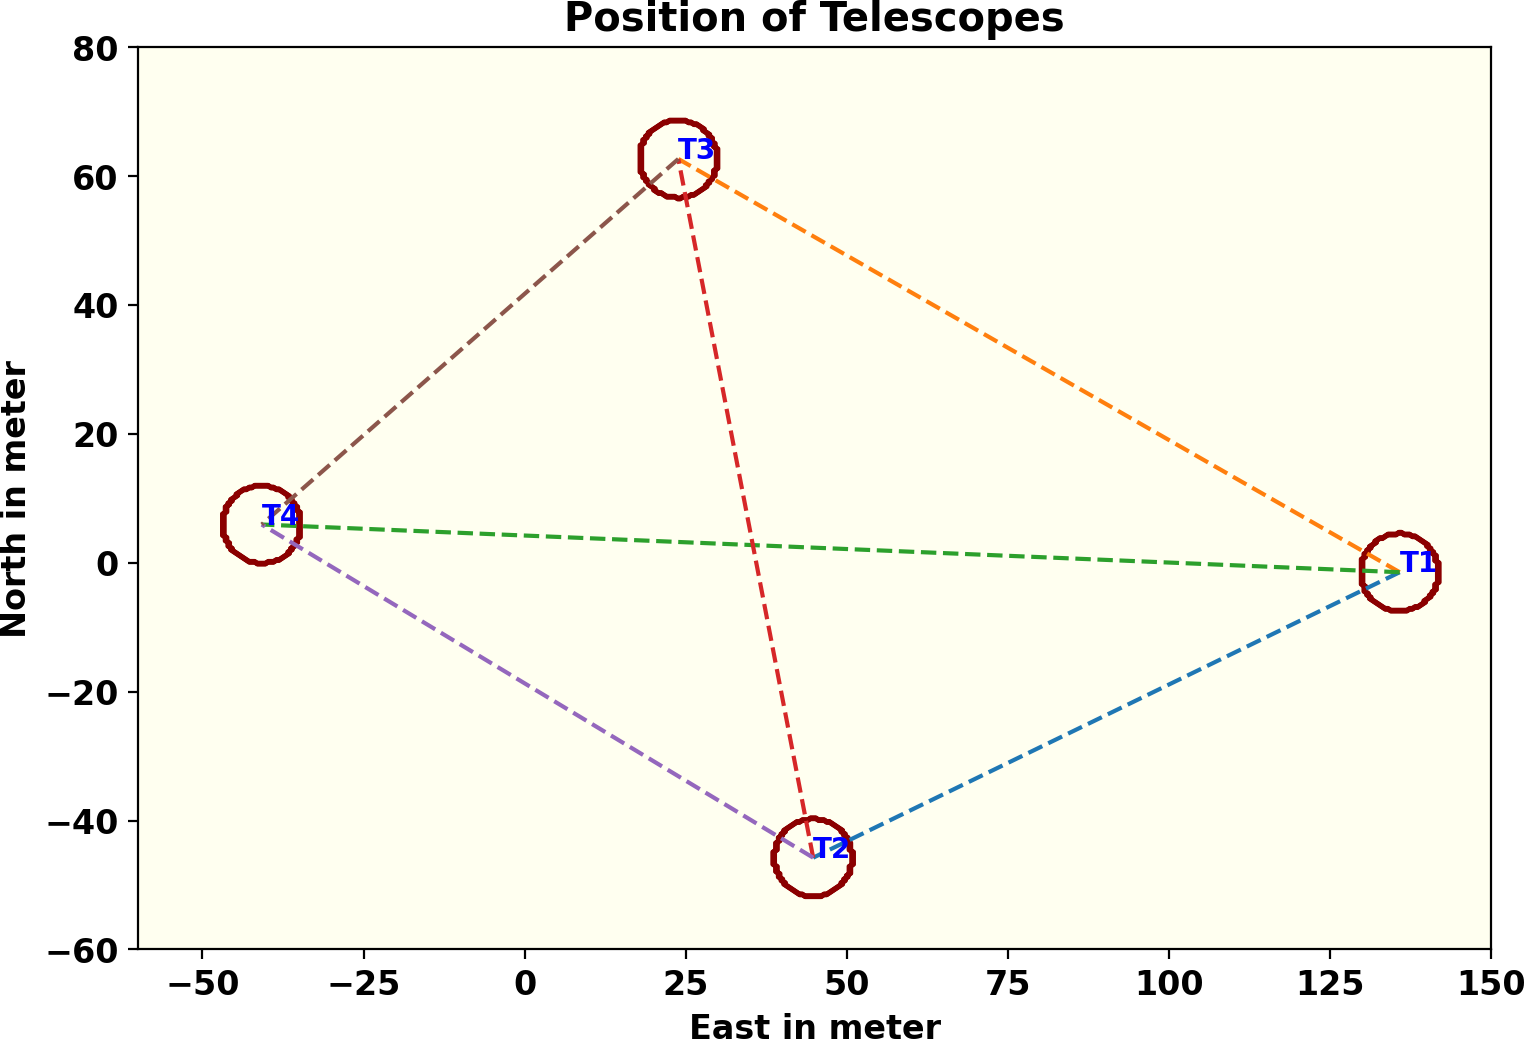
\includegraphics[width=\linewidth]{fig/telescope.png}
	\caption{The telescope configuration with similar properties each used to simulate the signal for II.}
	\label{fig:teles}
\end{figure}
\begin{figure}
	\centering
	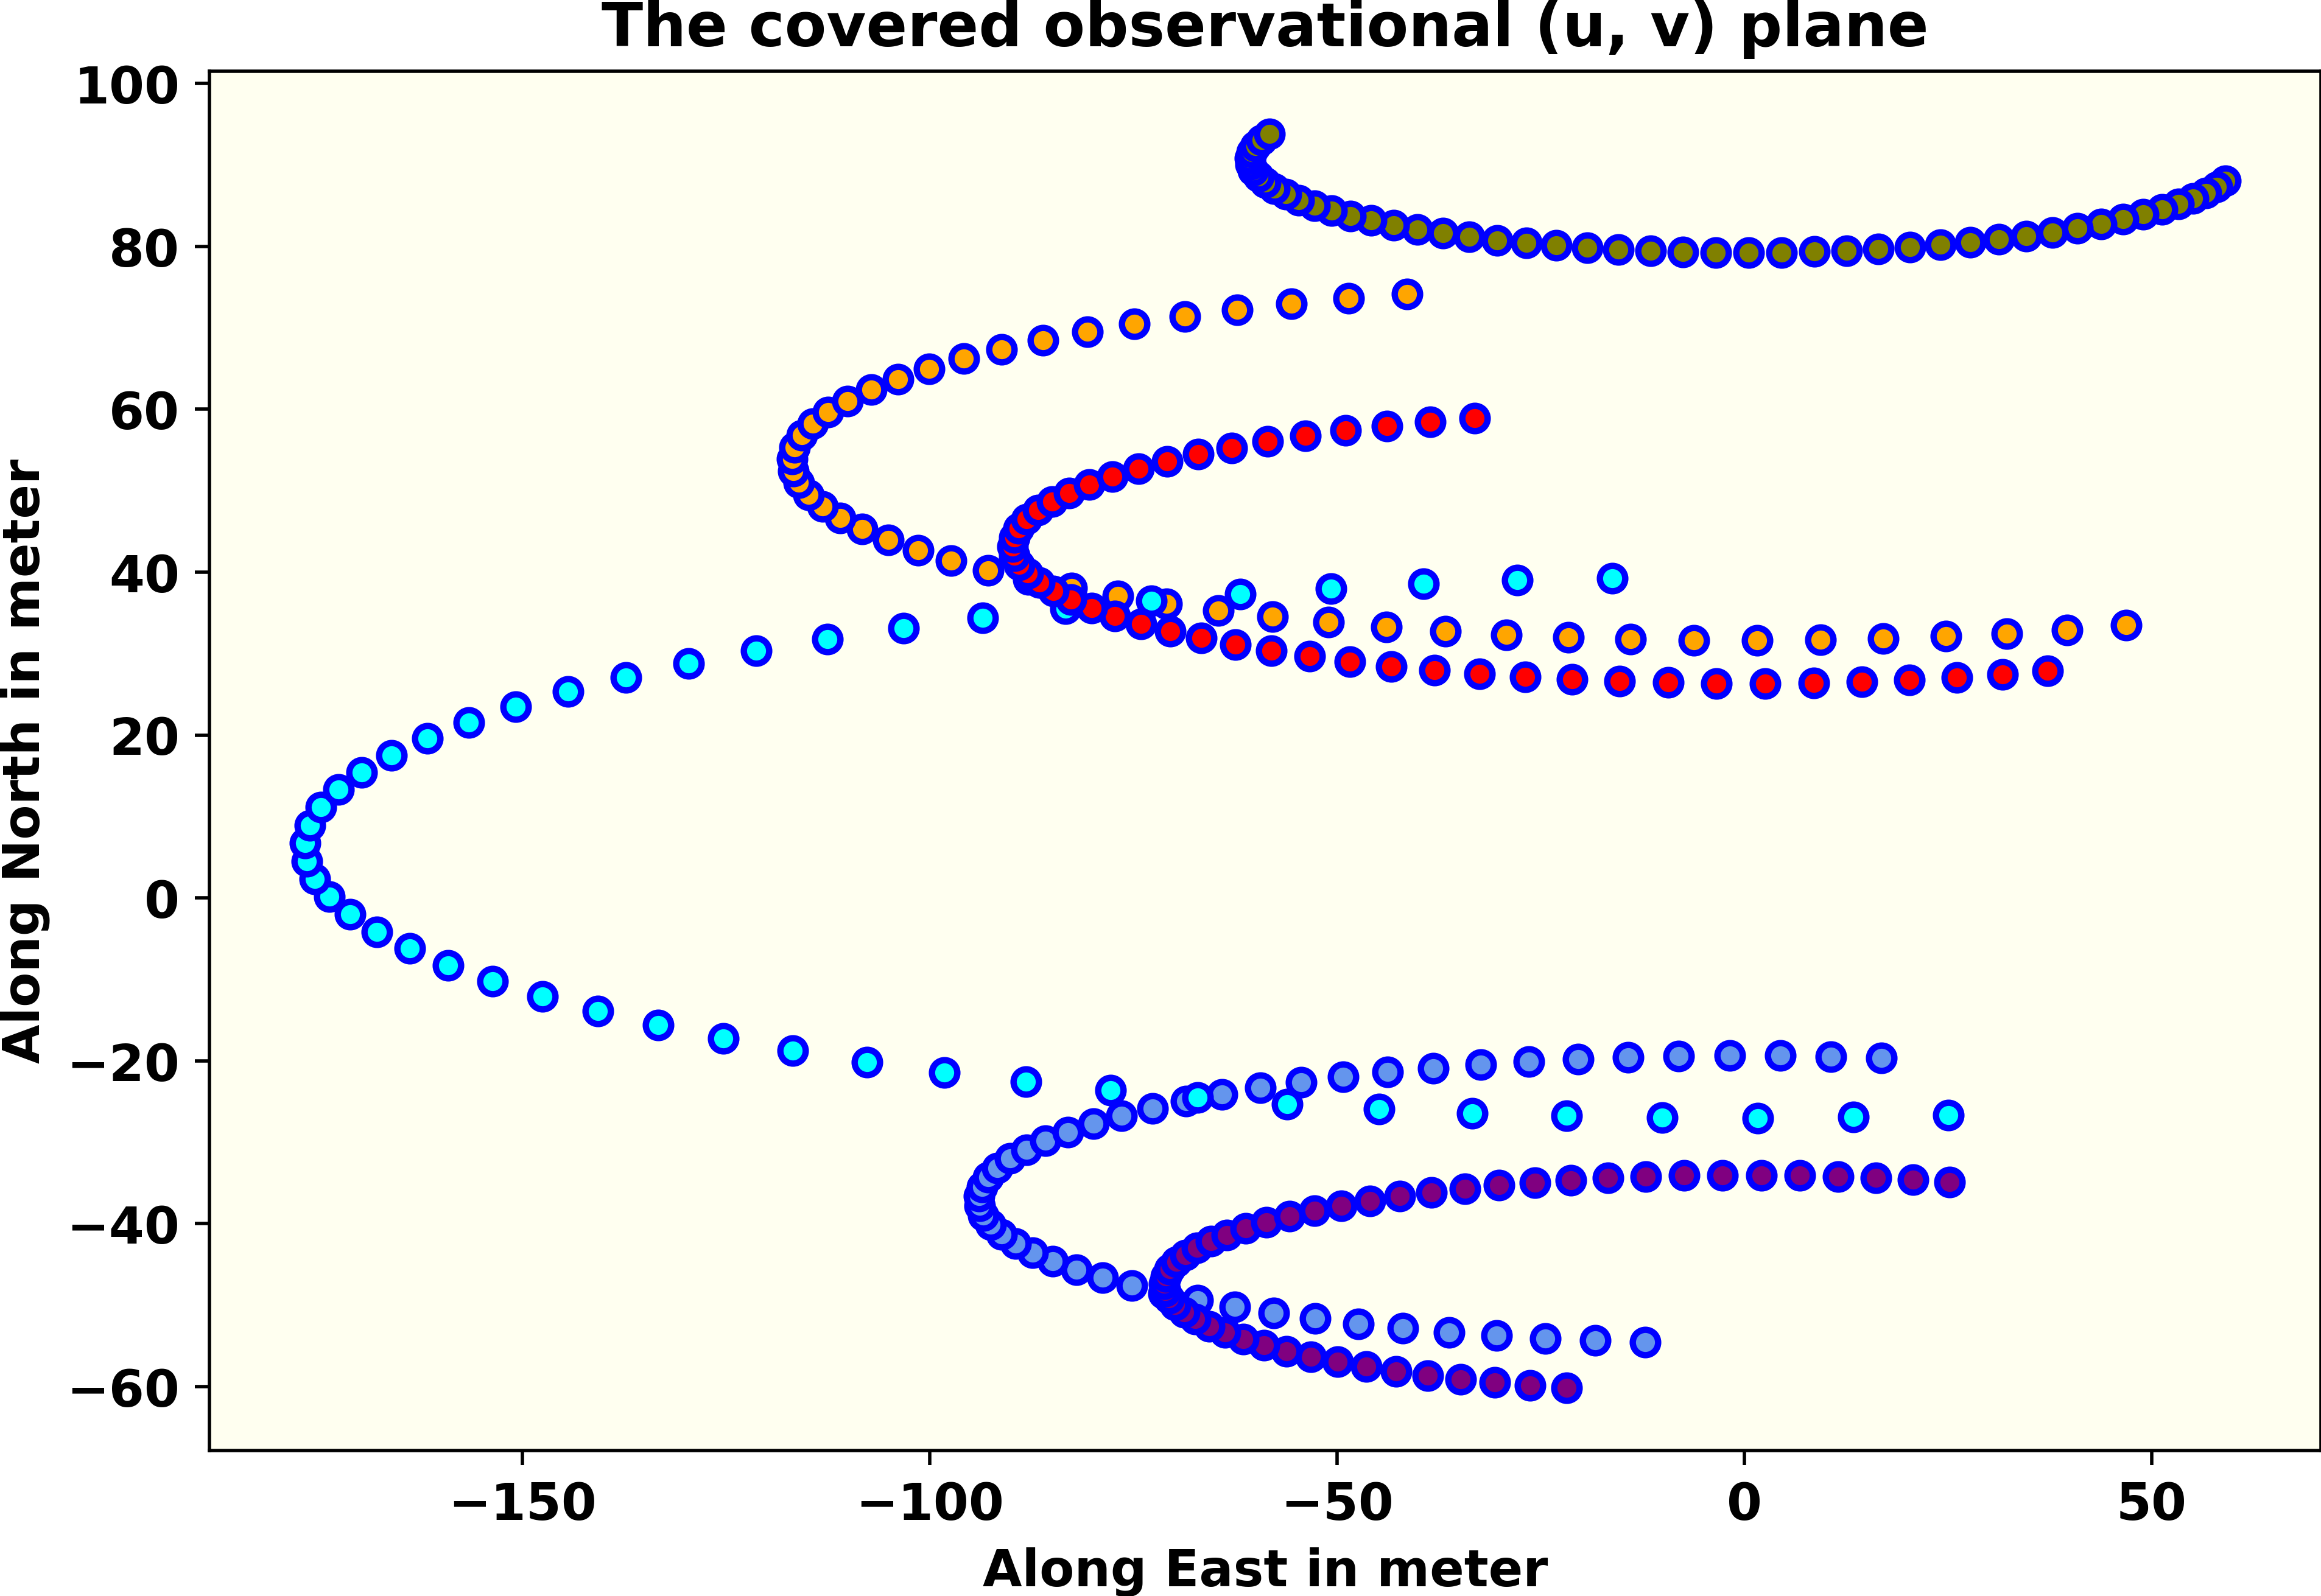
\includegraphics[width=\linewidth]{fig/baseline.png}
	\caption{The tracking of baselines with four telescopes arranged in fig.~\ref{fig:teles} for one night of observation.}
	\label{fig:base}
\end{figure}
\begin{figure}
	\centering
	\includegraphics[width=0.8\linewidth]{fig/ellipse/ellipse6018.jpg}
	\caption{This figure shows the simulated fast rotating star. The brightness is highest at the pole and there is gravitational darkening at the equator.}
	\label{fig:image}
\end{figure}
\begin{figure*}
	\centering
	\begin{subfigure}{0.5\linewidth}
		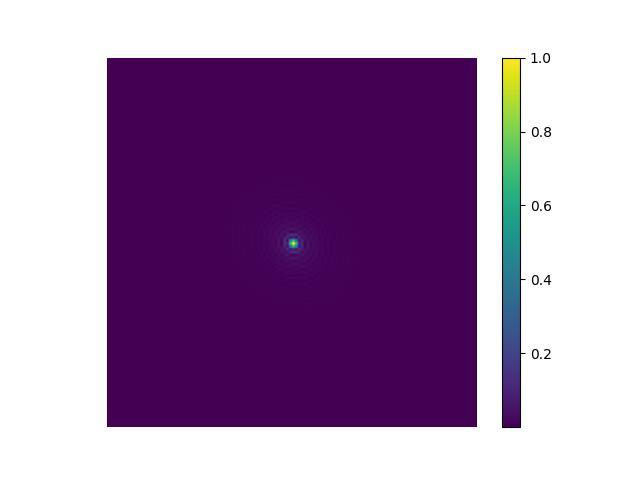
\includegraphics[width=\linewidth]{fig/ft/ft.jpg}
		\caption{The fourier transform of source.}
	\end{subfigure}\hfill
	\begin{subfigure}{0.5\linewidth}
		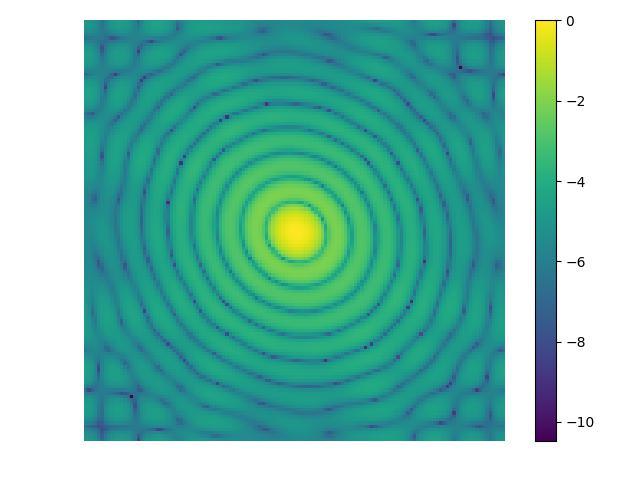
\includegraphics[width=\linewidth]{fig/ft/ft_log.jpg}
		\caption{The logarithmic fourier transform of source.}
	\end{subfigure}
	\caption{Absolute value of the two-dimensional Fast Fourier Transform of fig.~\ref{fig:image} measured by Intensity Interferometry, and observation of maximum (u, v) plane with finite number of baselines can be completed with help of earth's rotation.}
	\label{fig:ft}
\end{figure*}
\begin{figure*}
	\centering
	\begin{subfigure}{0.5\linewidth}
		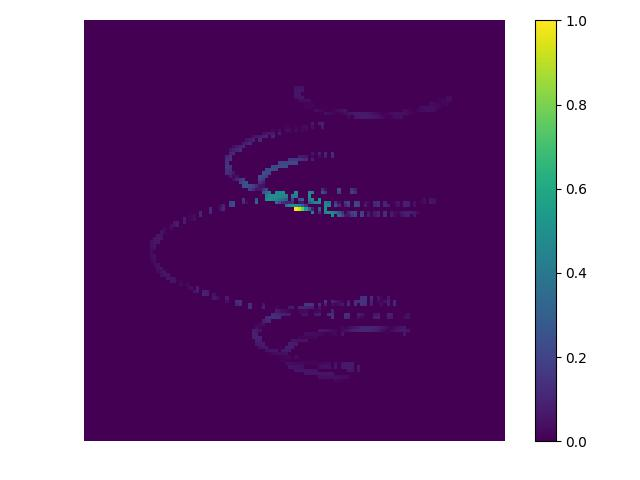
\includegraphics[width=\linewidth]{fig/ft/ft_base.jpg}
		\caption{The fourier transform with baselines.}
	\end{subfigure}\hfill
	\begin{subfigure}{0.5\linewidth}
		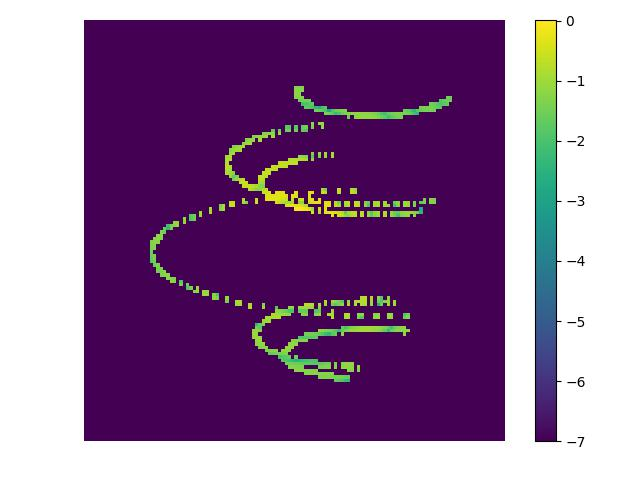
\includegraphics[width=\linewidth]{fig/ft/ft_log_base.jpg}
		\caption{The logarithmic fourier transform with baselines.}
	\end{subfigure}
	\caption{The left panel shows the absolute value of the two-dimensional Fast Fourier Transform of fig.~\ref{fig:image} measured by baselines shown in fig.~\ref{fig:teles}. The right panel shows the same on logarithmic scale}
	\label{fig:ft_base}
\end{figure*}
The primary purpose of IACTs is to study high-energy gamma rays (with energy $E\ \geq 30$ GeV) arriving from cosmic sources, entering the Earth's atmosphere, and initiating Cherenkov showers in the upper atmosphere due to multiple scattering. These telescopes feature an array of mirrors that focus light onto a set of photo-multiplier tubes (PMTs) \cite{aleksic2016major}. In the simulation model adopted here, we consider a set of four IACTs, each with similar properties. The positional configuration of these IACTs is shown in fig.~\ref{fig:teles}. The optical signal directed to a PMT is filtered using a spectral filter with a chosen mean observational wavelength $\lambda$ and corresponding bandpass $\Delta \lambda$. The use of filters not only reduces background noise but also improves the signal quality and the efficiency of the PMTs. Filtering background skylight becomes even more significant in II observations, as these are carried out during full moon nights. It is important to note that the light from the stellar source is focused on the PMT during II observations.

The significance of the signal can be expressed in terms of the signal-to-noise ratio (SNR), which depends on many factors. However, most importantly, it does not depend on the optical bandwidth $\Delta {\mathrm {\nu}}$ of the radiation for a two-telescope correlation. The explanation for the independence of the SNR from $\Delta {\mathrm {\nu}}$ is provided \DIFdelbegin \DIFdel{at the end of subsection 4.1 of \mbox{%DIFAUXCMD
\cite{10.1093/mnras/stab2391}}\hskip0pt%DIFAUXCMD
.  }\DIFdelend \DIFaddbegin \DIFadd{in several works \mbox{%DIFAUXCMD
\citep[e.g., subsection 4.1 of][]{10.1093/mnras/stab2391}}\hskip0pt%DIFAUXCMD
.  The Signal-to-Noise is given by
}\DIFaddend \begin{equation}
	SNR = A \cdot \alpha \cdot q \cdot n \cdot F^{-1} \cdot \sigma \cdot \sqrt{\frac{T \Delta f}{2}} \cdot \abs{V_{12}}^{2}
	\label{eq:SNR}
\end{equation}
Here, $A$ is the total mirror area, $\alpha$ is the quantum efficiency of the PMTs, $q$ is the \DIFdelbegin \DIFdel{quantum efficiency }\DIFdelend \DIFaddbegin \DIFadd{throughput }\DIFaddend of the remaining optics, and $n$ is the differential photon flux from the source. The excess noise factor of the PMTs is represented by $F$, $T$ denotes the observation time, and $\sigma$ is the normalized spectral distribution of the light (including filters) \DIFdelbegin \DIFdel{\mbox{%DIFAUXCMD
\cite{acciari2020optical}}\hskip0pt%DIFAUXCMD
}\DIFdelend \DIFaddbegin \DIFadd{\mbox{%DIFAUXCMD
\citep[e.g.,][]{acciari2020optical}}\hskip0pt%DIFAUXCMD
}\DIFaddend . The signal (S) and noise (N) can be understood using eqns.\ref{eq:signal} and \ref{eq:SNR} as:
\begin{equation}
	S = \frac{\Delta f}{\Delta \nu} \abs{V_{12}}^2
\end{equation}
and
\begin{equation}
	N = (A \cdot \alpha \cdot q \cdot n \cdot F \cdot \sigma \cdot \Delta \nu)^{-1}\sqrt{\frac{2 \Delta f}{T}}.
\end{equation}
While most of the parameters can be optimized with hardware, the only way to achieve a better SNR with fixed telescopes is to increase the observation time $T$.

\subsection{Baseline considerations}
The measurement of the size of stellar objects via absolute visibility depends on the distance between the telescopes, known as the baseline $d$.
\begin{equation}
	V_{12}(d) = \frac{c(d)}{c(0)}
	\label{eq:angular_size_meas}
\end{equation}
For achieving a good SNR with a given telescope configuration, covering \DIFdelbegin \DIFdel{the largest possible observational }\DIFdelend \DIFaddbegin \DIFadd{as much as possible of the interferometric }\DIFaddend plane is always desirable\DIFdelbegin \DIFdel{\mbox{%DIFAUXCMD
\citep{acciari2020optical, abeysekara2020demonstration}}\hskip0pt%DIFAUXCMD
}\DIFdelend . If the source is at the zenith, the coordinates in the Fourier plane ($u,v$) are given by:
\begin{equation}
	(u,v) = \frac{1}{\lambda} (d_E, d_N)
\end{equation}
where $d_E$ and $d_N$ are the baselines expressed in east and north coordinates. However, not all sources are at the zenith, and the telescopes are stationary and may also have different relative altitudes $d_A$ depending on the available terrain. Therefore, the Earth's rotation must be taken into account to cover the maximum observational plane using rotated baselines. For a given stellar source with declination $\delta$ and hour-angle $h$, as observed by telescopes at latitude $l$, equation (\ref{eq:baseline_rot}) provides the rotated baselines for a given pair of telescopes \DIFdelbegin \DIFdel{\mbox{%DIFAUXCMD
\citep{dravins2013optical, saha2020theory}}\hskip0pt%DIFAUXCMD
}\DIFdelend \DIFaddbegin \DIFadd{\mbox{%DIFAUXCMD
\citep[see e.g., eqs.~8--10 from][]{2020MNRAS.498.4577B}}\hskip0pt%DIFAUXCMD
}\DIFaddend .
\begin{equation}
\begin{pmatrix} u\\ v\\ w\\ \end{pmatrix} = R_x(\delta) \cdot R_y(h) \cdot R_x(-l) \begin{pmatrix} d_E \\ d_N \\ d_A \\ \end{pmatrix}
	\label{eq:baseline_rot}
\end{equation}

\DIFdelbegin \DIFdel{The three rotation matrices $R_i$ correspond to the fundamental representation of the SO(3) group \mbox{%DIFAUXCMD
\cite{saha2020theory}}\hskip0pt%DIFAUXCMD
. Fig.}\DIFdelend \DIFaddbegin \DIFadd{Fig.~}\DIFaddend \ref{fig:base} shows the track of six baselines generated from the telescopes (\DIFdelbegin \DIFdel{fig.}\DIFdelend \DIFaddbegin \DIFadd{Fig.~}\DIFaddend \ref{fig:teles}) due to \DIFaddbegin \DIFadd{the }\DIFaddend Earth's rotation. Since every pair of telescopes traces an ellipse in the Fourier plane, the total number of ellipses scales as
\DIFdelbegin \DIFdel{follows: 
}\DIFdelend \begin{equation}
	\label{eq:N_telescopes}
	\mathcal{N} = \DIFdelbegin \DIFdel{\frac{N_T \cdot (N_T -1)}{2}
}\DIFdelend \DIFaddbegin \tfrac12 \DIFadd{N_T \cdot (N_T -1)
}\DIFaddend \end{equation}
where $N_T$ is the number of telescopes considered.
As the number of baselines increases non-linearly, Intensity Interferometry (II) benefits greatly from a large number of telescopes. The planned Cherenkov Telescope Array (CTA) will cover the maximum observational plane and provide insight into stellar objects with optical wavelengths in the future.

\subsection{\DIFdelbegin \DIFdel{A }\DIFdelend Fast Rotating \DIFdelbegin \DIFdel{Star}\DIFdelend \DIFaddbegin \DIFadd{Stars}\DIFaddend : The \DIFdelbegin \DIFdel{Object in Our Instance}\DIFdelend \DIFaddbegin \DIFadd{Objects Considered}\DIFaddend }
In our work presented here, we simulate a single fast-rotating star to test image reconstruction using a GAN. Fast rotation causes stars to adopt an oblate shape, flattening at the poles and bulging at the equator due to the stronger centrifugal force \DIFdelbegin \DIFdel{\mbox{%DIFAUXCMD
\cite{von1924radiative, 1999A&A...347..185M}}\hskip0pt%DIFAUXCMD
}\DIFdelend \DIFaddbegin \DIFadd{\mbox{%DIFAUXCMD
\citep[e.g.,][]{von1924radiative, 1999A&A...347..185M}}\hskip0pt%DIFAUXCMD
}\DIFaddend . Fig.~\ref{fig:image} shows one of the simulations of such a fast-rotating star, with brightness distributed across its surface. The brightness is highest at the poles and lowest at the equator, a phenomenon known as gravity darkening \DIFdelbegin \DIFdel{\mbox{%DIFAUXCMD
\cite{lucy1967gravity}}\hskip0pt%DIFAUXCMD
}\DIFdelend \DIFaddbegin \DIFadd{\mbox{%DIFAUXCMD
\citep{lucy1967gravity}}\hskip0pt%DIFAUXCMD
}\DIFaddend . This effect was first observed through interferometric and spectroscopic data from the CHARA Array for the fast-rotating star Regulus \cite{mcalister2005first}. Fast-rotating stars are crucial for understanding various astrophysical processes, including stellar evolution, internal structure, and dynamical behavior over time.

Intensity Interferometry \DIFdelbegin \DIFdel{measures (or counts ) }\DIFdelend \DIFaddbegin \DIFadd{counts }\DIFaddend the photons arriving at the telescopes from the stellar object. The correlation of these photon arrivals at the telescopes yields the squared visibility (explained in subsection\DIFdelbegin \DIFdel{.}\DIFdelend \DIFaddbegin \DIFadd{~}\DIFaddend \ref{sec:signal}). \DIFdelbegin \DIFdel{According to Van Cittert Zernike's theorem, this }\DIFdelend \DIFaddbegin \DIFadd{This }\DIFaddend signal is the Fourier transform of the brightness distribution in the sky. Fig.\ref{fig:ft} represents the Fourier Transform of the source shown in \DIFdelbegin \DIFdel{fig.}\DIFdelend \DIFaddbegin \DIFadd{Fig.~}\DIFaddend \ref{fig:image} using II, displayed on both linear and logarithmic scales. In \DIFdelbegin \DIFdel{order to observe a real stellar source, however, one would need to receive photons from every point on the surface of the source, which would require an infinite number of baselines observing the source over a sufficiently long duration—an obviously unfeasible demand. In practice, we have a }\DIFdelend \DIFaddbegin \DIFadd{practice, only a small part of this information is available, because one has a }\DIFaddend finite number of baselines corresponding to the finite number $N_T$ of telescopes at our disposal and a limited observation schedule. Therefore, \DIFdelbegin \DIFdel{as a pilot, }\DIFdelend we have simulated the II observation of a sky source over one night\DIFdelbegin \DIFdel{'s duration}\DIFdelend . Using this finite amount of signal from one night's observation, we have trained a Generative Adversarial Network (GAN) to construct the image of the source.


\section{Generative Adversarial Networks}
\DIFdelbegin \DIFdel{In 2014, Ian Goodfellow introduced }\DIFdelend Generative Adversarial Networks (GANs) \DIFaddbegin \DIFadd{were introduced by \mbox{%DIFAUXCMD
\citep{goodfellow2014generative}}\hskip0pt%DIFAUXCMD
}\DIFaddend . The underlying concept is straightforward: it involves two competing networks. The first network, known as the Generator, produces new images based on an input image. \DIFdelbegin \DIFdel{For consistency, images produced by the Generator }\DIFdelend \DIFaddbegin \DIFadd{These }\DIFaddend will be referred to as generated images. The second network, the Discriminator, attempts to distinguish between the generated image (predicted image) and the real image (ground truth)\DIFdelbegin \DIFdel{\mbox{%DIFAUXCMD
\citep{goodfellow2014generative}}\hskip0pt%DIFAUXCMD
}\DIFdelend .

Through the alternating training of these networks, the generated images gradually become indistinguishable from the real images. Essentially, this process constitutes a two-player min-max game \DIFdelbegin \DIFdel{— }\DIFdelend \DIFaddbegin \DIFadd{--- }\DIFaddend a classic problem in game theory. The original formulation of GANs is given by:
\begin{equation}
	\centering
	\begin{aligned}
		\min_{G} \max_{D} V(D, G) &= \mathbb{E}_{x \sim p_{data}(x)} \left[ \log D(x) \right] \\
		&+ \mathbb{E}_{z \sim p_{z}(z)} \left[ \log \left( 1-D(G(z)) \right) \right]
	\end{aligned}
	\label{eq:Basic_GAN}
\end{equation}
where $V(D, G)$ denotes the value function of the min-max game.

The objective is to learn the Generator's distribution, \(p_G\), over the data \(x\). We begin with input noise variables \(p_z(z)\) and employ two perceptrons, \(G(z; \theta_G)\) and \(D(x; \theta_D)\), parameterized by \(\theta_i\) with \(i = G \ \mathrm{or}\ D\) respectively. Here, \(G(z)\) is a differentiable function that maps \(z\) to the data space \(x\), while \(D(x)\) represents the probability that \(x\) originates from real data\DIFdelbegin \DIFdel{\mbox{%DIFAUXCMD
\cite{goodfellow2014generative}}\hskip0pt%DIFAUXCMD
}\DIFdelend . The problem can be reformulated as:
\begin{equation}
	\centering
	\begin{aligned}
		\max_{D} V(G, D) &= \mathbb{E}_{x \sim p_{data}} \left[ \log D^{*}_{G}(x) \right] \\ 
		&+ \mathbb{E}_{x \sim p_{g}} \left[ \log \left( 1 - D^{*}_{G}(x) \right) \right]
	\end{aligned}
	\label{eq:GAN_reformulated}
\end{equation}
where \(D^{*}_{G}\) denotes the optimum of the discriminator for a given fixed generator, as shown in equation (\ref{eq:Disc_optimum}). It can be demonstrated that the global optimum of equation (\ref{eq:GAN_reformulated}) is achieved if and only if \(p_G = p_{data}\). Furthermore, if both \(G\) and \(D\) are allowed to reach their respective optima, then \(p_G\) converges to \(p_{data}\). A more comprehensive discussion of the problem, including proofs, is provided in \DIFdelbegin \DIFdel{\mbox{%DIFAUXCMD
\citep{goodfellow2014generative}}\hskip0pt%DIFAUXCMD
}\DIFdelend \DIFaddbegin \DIFadd{\mbox{%DIFAUXCMD
\cite{goodfellow2014generative}}\hskip0pt%DIFAUXCMD
}\DIFaddend .
\begin{equation}
	\centering
	D^*_G(x) = \frac{p_{data}(x)}{p_{data}(x) + p_g(g)}
	\label{eq:Disc_optimum}
\end{equation}
\begin{figure}
	\centering
	\includegraphics[width=\linewidth]{fig/ellipsoid_0.jpg}
	\caption{Merged image, which includes the original and the sparsely sampled Fourier plane. It is exactly what the GAN receives. }
	\label{fig:GANinput}
\end{figure}
\begin{figure}
	\centering
	\begin{subfigure}{\linewidth}
		\centering
		\includegraphics[width=\textwidth]{fig/analysis/Plot_learning_rate_disc_loss.pdf}
		\caption{Discriminator loss for three different learning rates. }
		\label{fig:Plot_learning_rate_discloss}
	\end{subfigure}\hfill
	\begin{subfigure}{\linewidth}
		\centering
		\includegraphics[width=\textwidth]{fig/analysis/Plot_learning_rate_gen_total_loss.pdf}
		\caption{Total generator loss for different learning rates (eqn. (\ref{eq:total_gen_loss})).}
		\label{fig:Plot_learning_rate_genloss}
	\end{subfigure}\hfill
	\caption{Generator and discriminator losses for three different learning rates. The upper figure shows the total discriminator loss, and the lower figure shows the total generator loss. There is no significant difference, but the highest learning rate might be prone to outliers. }
	\label{fig:Plot_learning_rate_loss}
\end{figure}
\begin{figure}
	\centering
	\begin{subfigure}{\linewidth}
		\centering
		\includegraphics[width=\textwidth]{fig/analysis/Plot_Kernel_size_disc_loss.pdf}
		\caption{Discriminator loss for three different kernel sizes. }
		\label{fig:Plot_kernel_size_discloss}
	\end{subfigure}\hfill
	\begin{subfigure}{\linewidth}
		\centering
		\includegraphics[width=\textwidth]{fig/analysis/Plot_Kernel_size_gen_total_loss.pdf}
		\caption{Total generator loss for three different kernel sizes.}
		\label{fig:Plot_kernel_size_genloss}
	\end{subfigure}\hfill
	\caption{Generator and discriminator losses for three different kernel sizes in the convolutional layers. Here, the smallest kernel size has many outliers, while the largest kernel size seems to be the most stable.}
	\label{fig:Plot_kernel_size_loss}
\end{figure}
\begin{figure*}
	\centering
	\begin{subfigure}{0.5\linewidth}
		\centering
		\includegraphics[width=\textwidth]{fig/analysis/Plot_noise_factor_disc_loss.pdf}
		\caption{Discriminator loss for different noise percentages.}
		\label{fig:Plot_noise_discloss}
	\end{subfigure}\hfill
	\begin{subfigure}{0.5\linewidth}
		\centering
		\includegraphics[width=\textwidth]{fig/analysis/Plot_noise_factor_gen_total_loss.pdf}
		\caption{Generator losses for different noise percentages.}
		\label{fig:Plot_noise_genloss}
	\end{subfigure}\hfill
	\caption{Effect of the Salt and Pepper noise introduced in the images. Different ratios between $\alpha$ and $\beta$ are shown. There is no significant effect. Please note that these results are from training on 64-pixel images.}
	\label{fig:Plot_noise_loss}
\end{figure*}
\begin{figure*}
	\centering
	\begin{subfigure}{0.5\linewidth}
		\centering
		\includegraphics[width=\textwidth]{fig/analysis/Plot_Batchsize_disc_loss.pdf}
		\caption{Discriminator loss for different batch sizes.}
		\label{fig:Plot_batchsize_discloss}
	\end{subfigure}\hfill
	\begin{subfigure}{0.5\linewidth}
		\centering
		\includegraphics[width=\textwidth]{fig/analysis/Plot_Batchsize_gen_total_loss.pdf}
		\caption{Generator losses for different batch sizes.}
		\label{fig:Plot_batchsize_genloss}
	\end{subfigure}\hfill
	\caption{Loss functions for two different batch sizes. Large batch sizes seem to be more robust, but they also increase training time significantly. }
	\label{fig:Plot_batchsize_loss}
\end{figure*}
\begin{figure*}
	\centering
	\begin{subfigure}{0.5\linewidth}
		\centering
		\includegraphics[width=\textwidth]{fig/analysis/Plot_Disc_rep_disc_loss.pdf}
		\caption{Discriminator loss for different Discriminator training.}
		\label{fig:Plot_discrep_discloss}
	\end{subfigure}\hfill
	\begin{subfigure}{0.5\linewidth}
		\centering
		\includegraphics[width=\textwidth]{fig/analysis/Plot_Disc_rep_gen_total_loss.pdf}
		\caption{Generator losses for different Discriminator training.}
		\label{fig:Plot_discrep_genloss}
	\end{subfigure}\hfill
	\caption{The amount of Discriminator training has a high impact on the Discriminator score. The Discriminator repetition indicates the factor by which the Discriminator is trained more with respect to the Generator.}
	\label{fig:Plot_discrep_loss}
\end{figure*}
\begin{figure*}
	\centering
	\begin{subfigure}{0.5\linewidth}
		\centering
		\includegraphics[width=\textwidth]{fig/analysis/Plot_N_telescopes_disc_loss.pdf}
		\caption{Discriminator loss for different amounts of telescopes.}
		\label{fig:Plot_telescopes_discloss}
	\end{subfigure}\hfill
	\begin{subfigure}{0.5\linewidth}
		\centering
		\includegraphics[width=\textwidth]{fig/analysis/Plot_N_telescopes_gen_total_loss.pdf}
		\caption{Generator loss for different amount of telescopes.}
		\label{fig:Plot_telescopes_genloss}
	\end{subfigure}\hfill
	\caption{The number of telescopes has a very impact on the model performance. If there are only two telescopes (1 baseline), both Discriminator and Generator are not trained smoothly: One gains a big advantage over the other. The result of four telescopes (6 baselines) is a lot better because the loss functions change only slightly with increasing steps.}
	\label{fig:Plot_telescopes_loss}
\end{figure*}

Subsequently, the GAN framework was extended to a conditional model \DIFdelbegin \DIFdel{\mbox{%DIFAUXCMD
\cite{mirza2014conditional}}\hskip0pt%DIFAUXCMD
}\DIFdelend \DIFaddbegin \DIFadd{\mbox{%DIFAUXCMD
\citep{mirza2014conditional}}\hskip0pt%DIFAUXCMD
}\DIFaddend . In this formulation, both the Generator and the Discriminator receive additional information \DIFdelbegin \DIFdel{\(y\)}\DIFdelend \DIFaddbegin \DIFadd{$y$}\DIFaddend , and the value function of the conditional GAN (cGAN) is expressed as:
\begin{equation}
	\centering
	\begin{aligned}
		V(D, G) &= \mathbb{E}_{x \sim p_{data}(x)} \left[ \log D(x|y) \right] \\
		&+ \mathbb{E}_{z \sim p_{z}(z)} \left[ \log \left( 1-D(G(z|y) \right) \right]
	\end{aligned}
	\label{eq:conditional_GAN}
\end{equation}

\DIFdelbegin \DIFdel{Furthermore, \mbox{%DIFAUXCMD
\cite{isola2017image} }\hskip0pt%DIFAUXCMD
}\DIFdelend \DIFaddbegin \DIFadd{\mbox{%DIFAUXCMD
\cite{isola2017image} }\hskip0pt%DIFAUXCMD
further }\DIFaddend observed that combining the cGAN from equation \ref{eq:conditional_GAN} with the traditional L1 loss improves the results, as the Generator is encouraged to produce outputs closer to the ground truth. Hence, the function that is minimized is:
\begin{equation}
	\centering
	L_{tot} = \arg \min_{G} \max_{D} V(D, G) + \lambda \cdot L_1(G)
	\label{eq:total_gen_loss}
\end{equation}
where $\lambda$ = 100 and $L_1(G)$ is given as
\begin{equation}
	\centering
	L_1(G) = \mathbb{E}_{x,y,z} \left[ ||{y - G(x,z)}||_1 \right]
	\label{eq:l1_loss}
\end{equation}

This type of network has demonstrated remarkable robustness across a variety of applications. For example, it can generate colored images from grayscale inputs based on architectural labels, transform images from day to night, and even predict maps from satellite data. A more extensive list of applications is provided in \cite{isola2017image}.


\subsection{Generator}
As discussed above, in a GAN the Generator is responsible for producing synthetic data—in this case, images that resemble those of a fast-rotating star. In this work, the Generator is implemented as a U-Net convolutional network \DIFdelbegin \DIFdel{\mbox{%DIFAUXCMD
\cite{ronneberger2015u}}\hskip0pt%DIFAUXCMD
}\DIFdelend \DIFaddbegin \DIFadd{\mbox{%DIFAUXCMD
\citep{ronneberger2015u}}\hskip0pt%DIFAUXCMD
}\DIFaddend . In such architectures, the image's spatial resolution is first reduced through downsampling and then restored via upsampling, resulting in a U-shaped structure. The downsampling process typically involves convolutional layers followed by a strided operation (with a stride of 2) to effectively subsample the image, and a leaky version of the Rectified Linear Unit (ReLU) is employed as the activation function.

In contrast, the upsampling process uses only the standard Rectified Linear Unit (ReLU) for neuron activation. This stage also comprises convolutional layers followed by operations with a stride of 2 to upscale the image to a higher resolution. Additionally, a dropout layer is introduced at the beginning of the upsampling phase to mitigate overfitting of the Generator model \cite{isola2017image}.

After generating images, the Generator aims to deceive the Discriminator into classifying the generated images as real. The extent to which the Generator succeeds in this deception is quantified by the GAN loss. When the Discriminator is unable to distinguish between the generated and real images (i.e., when the GAN loss is minimized), the Generator is considered to have reached an optimal state. Conversely, if the generated image fails to fool the Discriminator, the Generator produces a new image for further comparison with the real image. Additionally, the Generator's performance is evaluated using another metric known as the L1 loss, which is defined as the mean absolute error between the pixels of the real image and those of the generated image. Balancing the minimization of both the GAN loss and the L1 loss enables the Generator to produce images that are not only realistic but also faithful to the input data. 

\subsection{Discriminator}
As discussed earlier, the Discriminator is tasked with classifying the images produced by the Generator as either real or fake. It takes a real image from the dataset (often referred to as the target image for the Generator) and provides feedback to guide the Generator toward producing more accurate images. In this work, the PatchGAN model \cite{isola2017image} is employed as the Discriminator. Unlike a traditional global classifier, PatchGAN evaluates individual patches of the image, outputting a grid of predictions rather than a single scalar value.

The Discriminator’s architecture begins with an initializer that accepts both the input (generated) images and the corresponding real images. Initially, Salt-and-Pepper noise is added to the input images. PatchGAN then reduces the spatial dimensions of the images to extract localized features, ensuring the model focuses on smaller regions. In this downsampling stage, a leaky version of the Rectified Linear Unit (LeakyReLU) is applied in the convolutional layers, similar to the approach used in the Generator.

Subsequently, zero padding is applied—adding rows and columns of zeros around the images—to prevent the loss of spatial information during convolution and to facilitate the extraction of deeper features from the downsampled output. Following this, batch normalization is employed to stabilize learning by normalizing activations, and the Discriminator begins classifying each patch as real or fake. This is followed by additional layers involving LeakyReLU activation, zero padding, and convolution, culminating in a final prediction that the Generator uses as feedback.

The effectiveness of the Discriminator is measured by its ability to distinguish between real and fake images, quantified through the Discriminator loss. This loss is composed of two parts: one that measures how accurately the Discriminator identifies real images (by comparing predictions to a target value of 1) and another that assesses how accurately it identifies fake images (by comparing predictions to a target value of 0). Together, these loss components ensure that the Discriminator improves its classification performance, which in turn challenges the Generator to produce increasingly realistic images.
\DIFdelbegin \section{\DIFdel{The Parameter for GAN Structure}}
%DIFAUXCMD
\addtocounter{section}{-1}%DIFAUXCMD
\DIFdelend 

\DIFaddbegin \section{\DIFadd{Network Parameters}}

\DIFaddend \begin{figure*}
	\centering
	\begin{subfigure}{\linewidth}
		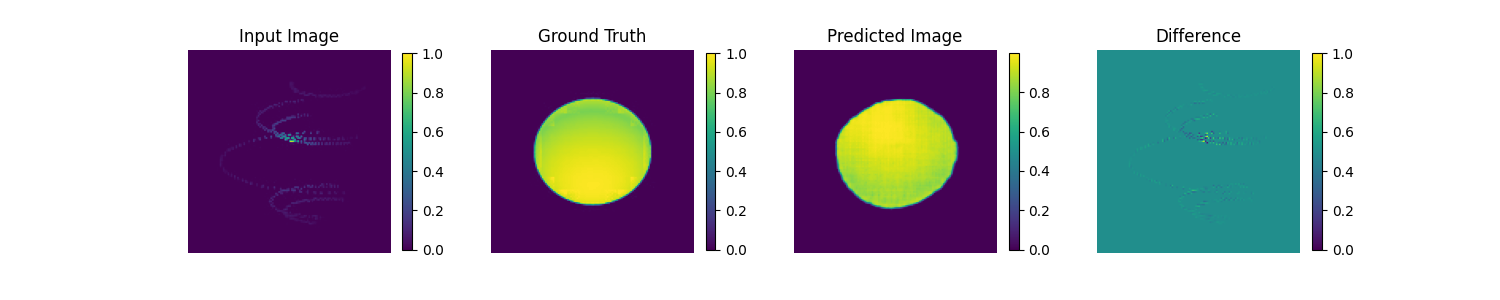
\includegraphics[width=\linewidth]{fig/testing_image/image_0.png}
	\end{subfigure}
	\begin{subfigure}{\linewidth}
		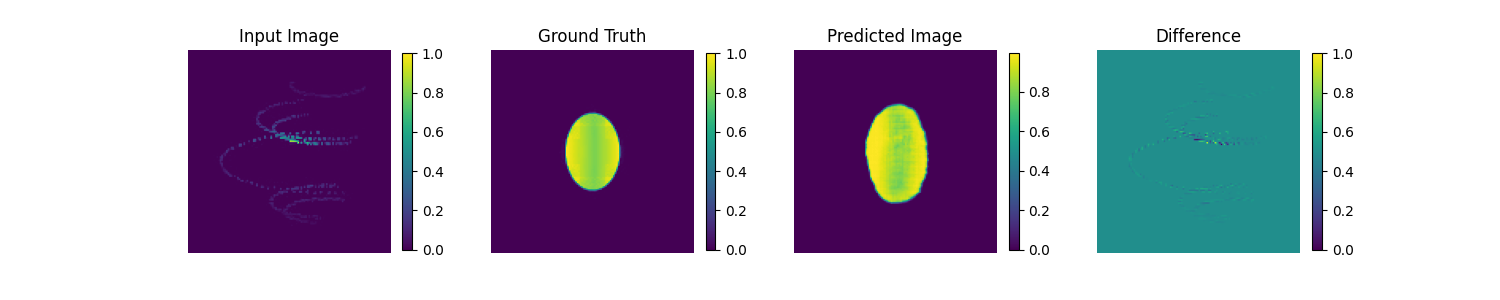
\includegraphics[width=\linewidth]{fig/testing_image/image_16.png}
	\end{subfigure}
	\begin{subfigure}{\linewidth}
		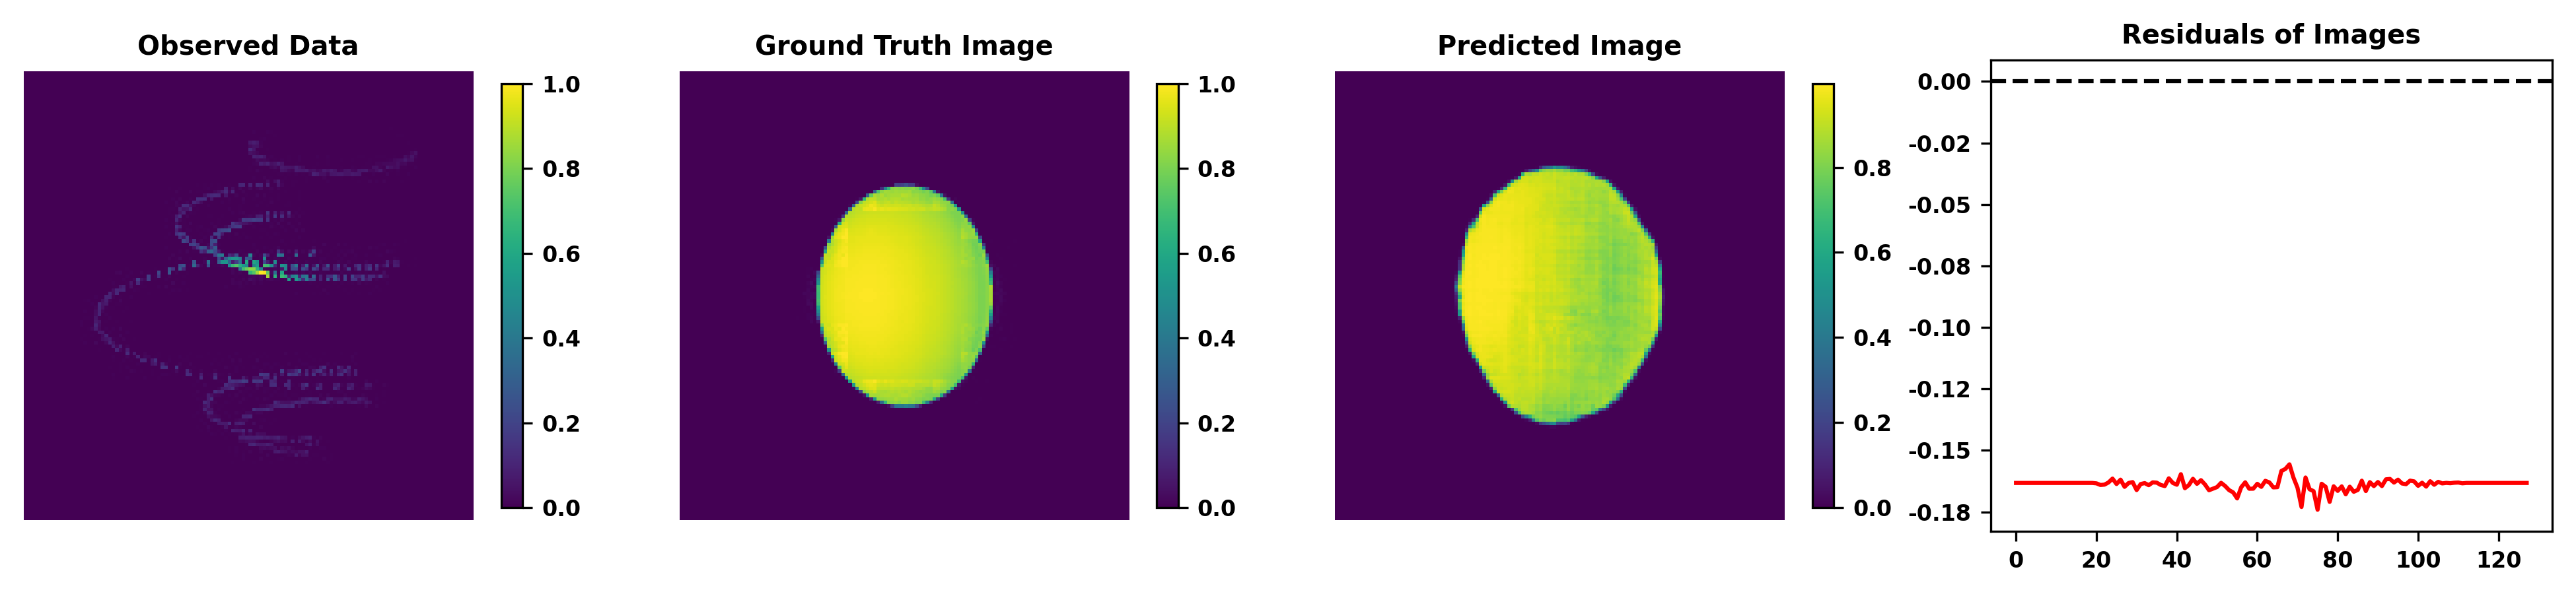
\includegraphics[width=\linewidth]{fig/testing_image/image_35.png}
	\end{subfigure}
	\begin{subfigure}{\linewidth}
		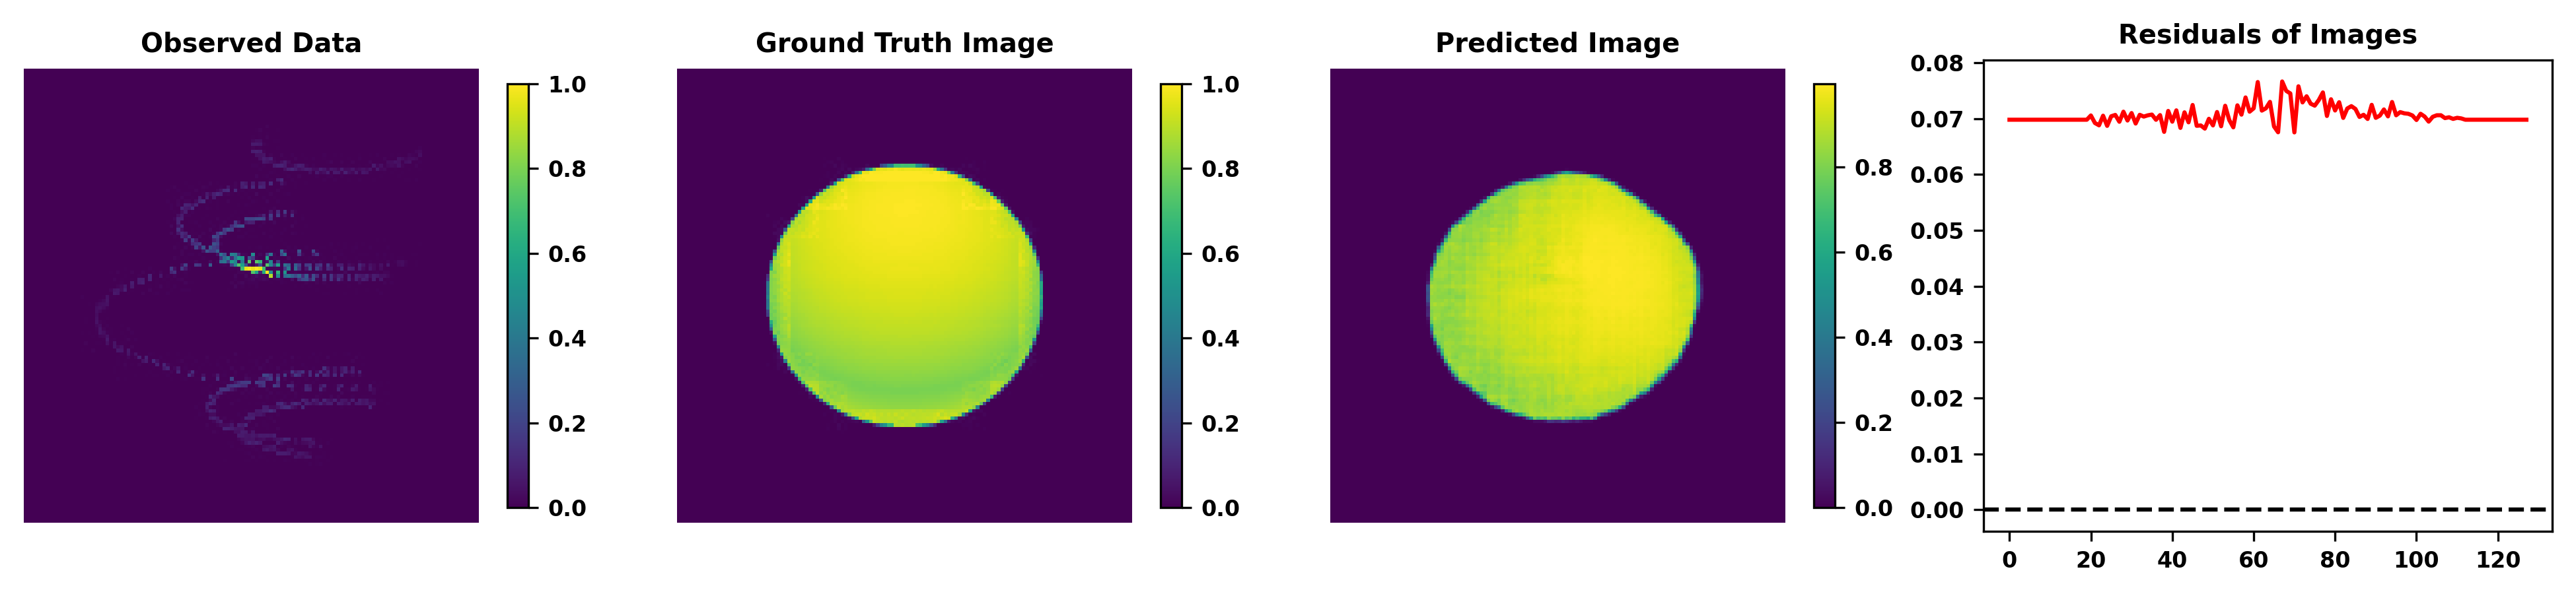
\includegraphics[width=\linewidth]{fig/testing_image/image_38.png}
	\end{subfigure}
	\begin{subfigure}{\linewidth}
		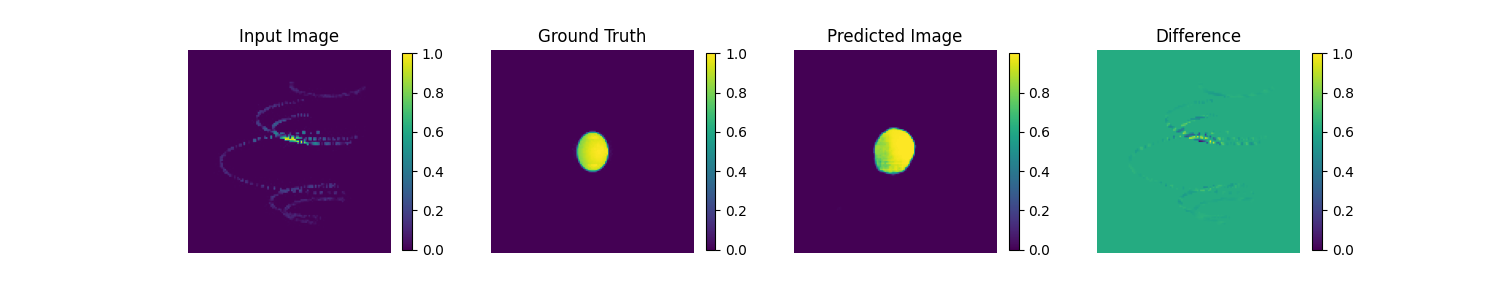
\includegraphics[width=\linewidth]{fig/testing_image/image_42.png}
	\end{subfigure}
	\begin{subfigure}{\linewidth}
		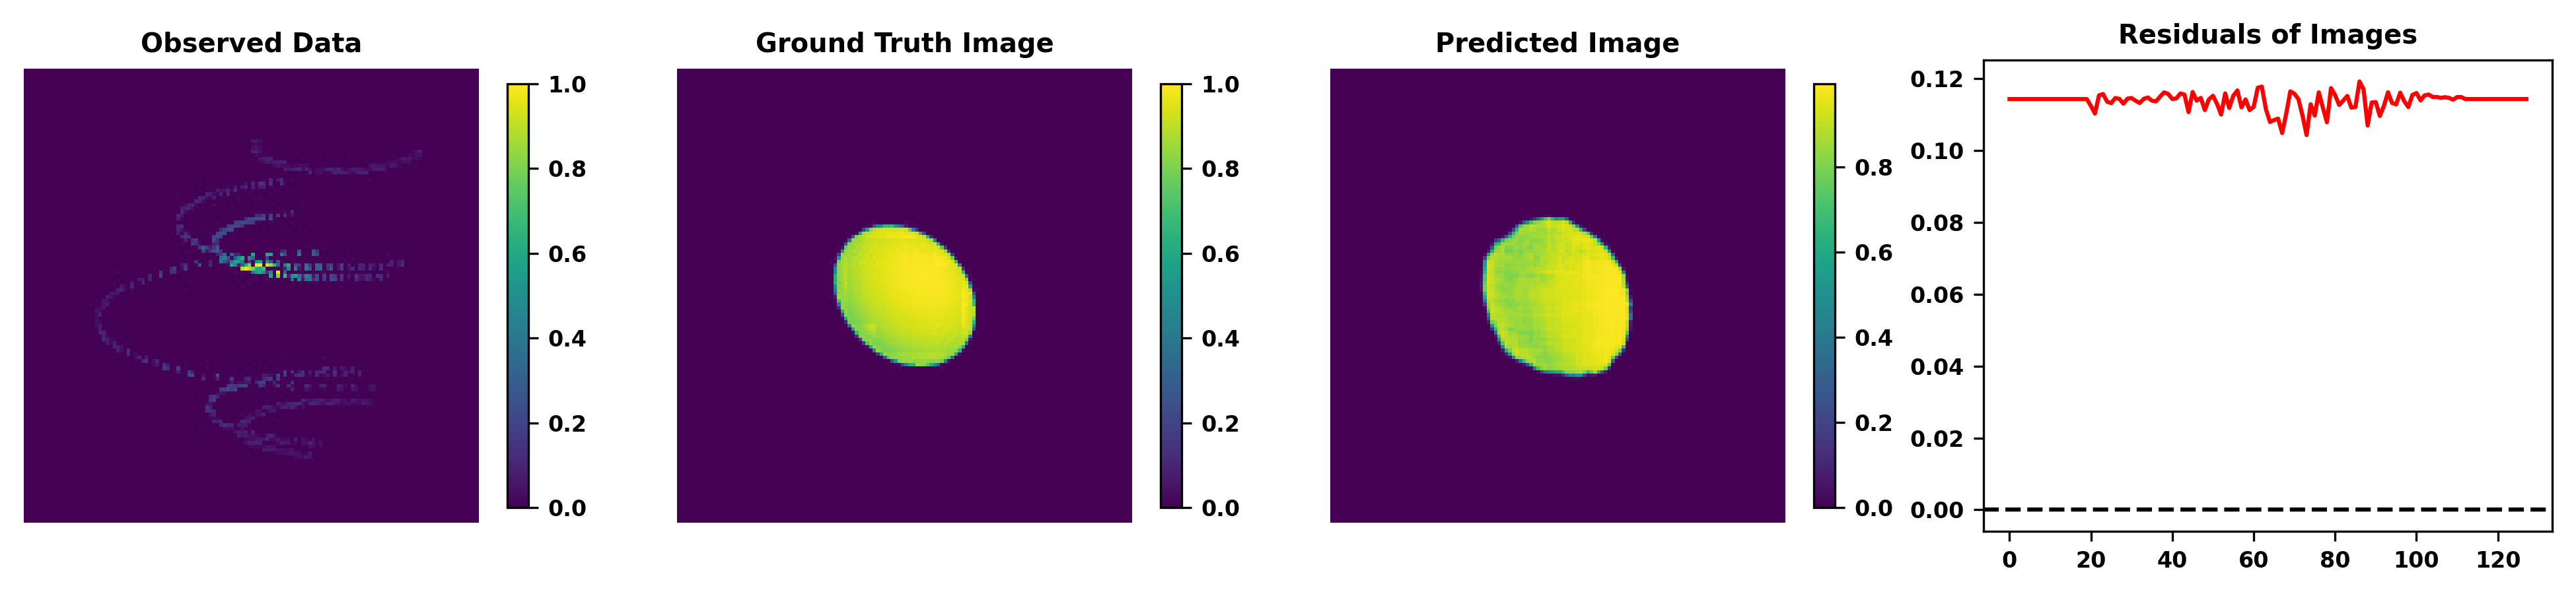
\includegraphics[width=\linewidth]{fig/testing_image/image_47.png}
	\end{subfigure}
	\caption{This set of figures shows the result of GAN for II. The left panels are signals using six baselines, which work as input for GAN. The first middle panel is the real image, also called ground truth, and GAN tries to mimic it during the training. The second middle panel is the reconstructed image, also called the predicted image, with trained GAN, and the end panel is the difference between the ground truth and the predicted image.}
	\label{fig:GAN}
\end{figure*}
Here, we discuss the parameters of the GAN architecture used for reconstructing images of stellar objects using II. Given the adversarial nature of GANs—where the Generator and Discriminator engage in a min-max game—careful tuning of key parameters is critical to ensure that both networks are well-balanced for effective training.

\subsection{Data Preparation}
First, we simulate fast-rotating stars, modeling them as oblate spheroids with varying radii and an oblateness ranging between 0.5 and 1. We also consider different viewing angles, assuming a linear dependence for the effect of gravity darkening. The traced ellipses result from integrating over the source's hour angle. For hyperparameter tuning and comparing different telescopes, the total \DIFdelbegin \DIFdel{hour angle }\DIFdelend \DIFaddbegin \DIFadd{observing duration }\DIFaddend is set to approximately 11.5 hours. Finally, the ellipses are plotted, converted into grayscale images, resized, and stored as raw arrays to facilitate further analysis.
\begin{figure*}
	\centering
	\begin{subfigure}{0.33\linewidth}
		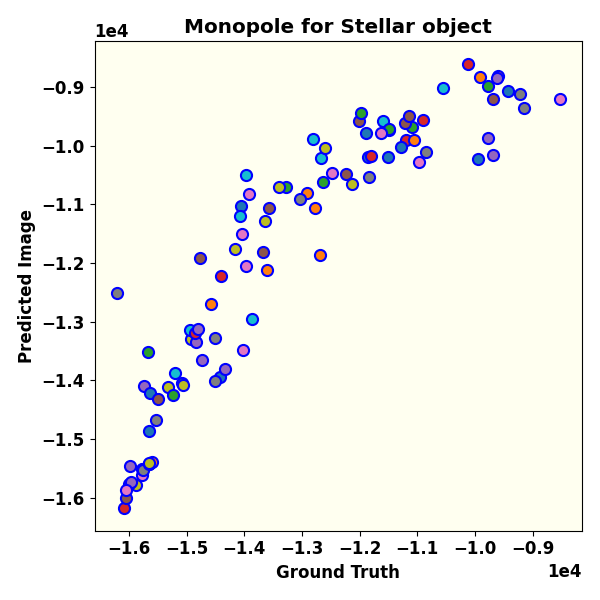
\includegraphics[width=\linewidth]{fig/moments/mom0.png}
		\caption{The monopole.}
		\label{fig:mom1}
	\end{subfigure}\hfill
	\begin{subfigure}{0.33\linewidth}
		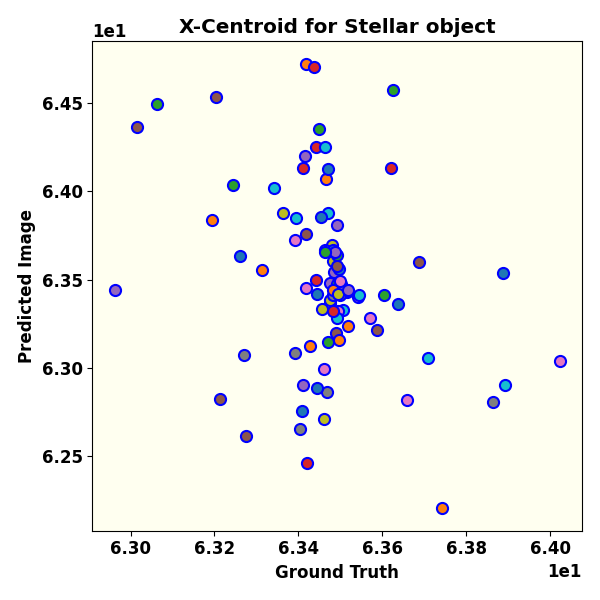
\includegraphics[width=\linewidth]{fig/moments/mom1.png}
		\caption{The centroids along x direction.}
		\label{fig:mom2}
	\end{subfigure}\hfill
	\begin{subfigure}{0.33\linewidth}
		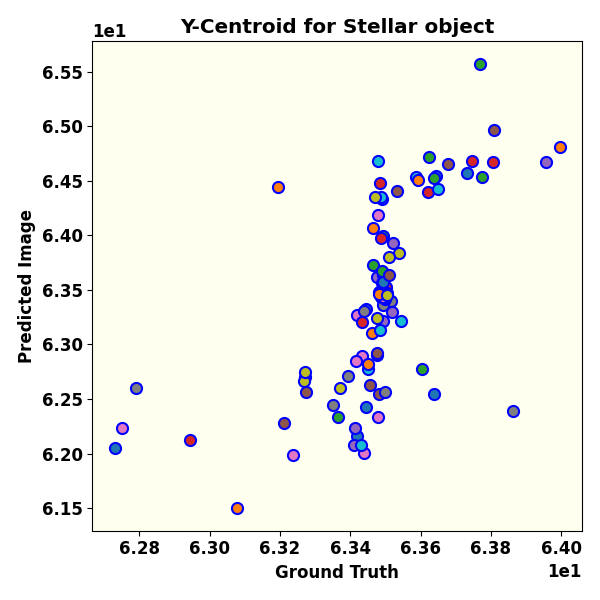
\includegraphics[width=\linewidth]{fig/moments/mom2.png}
		\caption{The centroids along y direction.}
		\label{fig:mom3}
	\end{subfigure}\hfill
	\caption{This set of figures shows the comparison of monopole, x-centroid, and y-centroid for ground truth and predicted images generated by trained GAN.}
	\label{fig:cen}
\end{figure*}
\begin{figure*}
	\centering
	\begin{subfigure}{0.33\linewidth}
		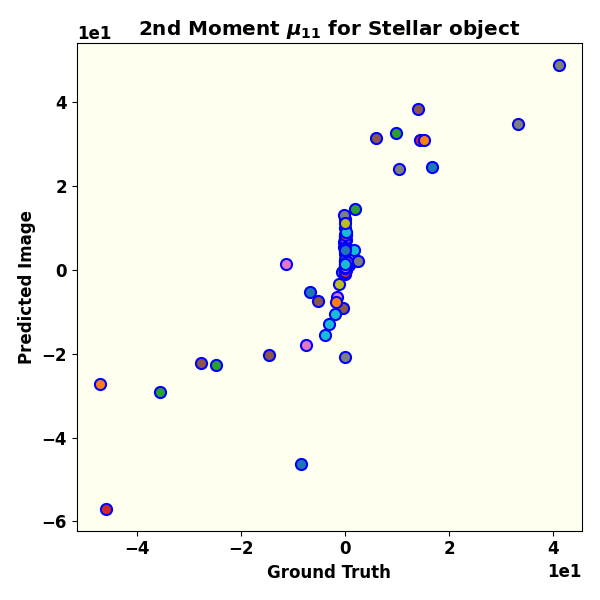
\includegraphics[width=\linewidth]{fig/moments/mom3.png}
		\caption{The 2nd order moment $\mu_{11}$.}
		\label{fig:mom4}
	\end{subfigure}\hfill
	\begin{subfigure}{0.33\linewidth}
		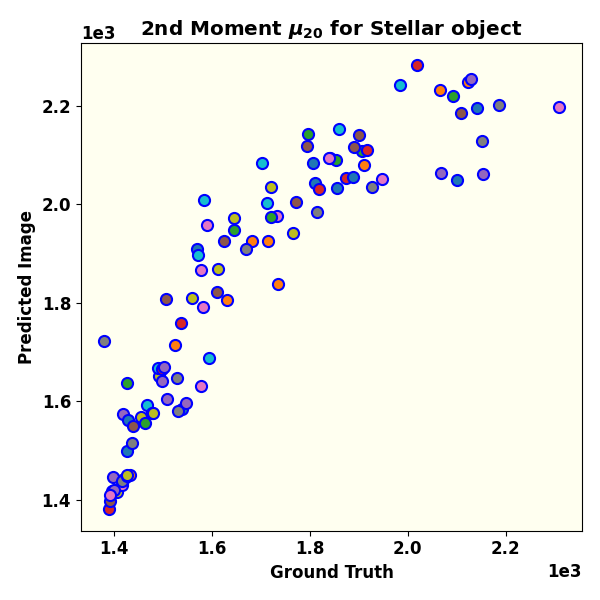
\includegraphics[width=\linewidth]{fig/moments/mom4.png}
		\caption{The 2nd order moment $\mu_{20}$.}
		\label{fig:mom5}
	\end{subfigure}\hfill
	\begin{subfigure}{0.33\linewidth}
		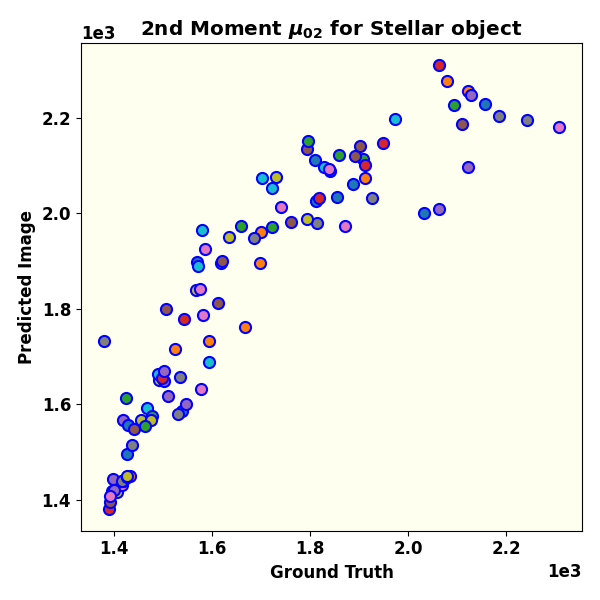
\includegraphics[width=\linewidth]{fig/moments/mom5.png}
		\caption{The 2nd order moment $\mu_{02}$.}
		\label{fig:mom6}
	\end{subfigure}\hfill
	\caption{The second-order central moments provide information about the size and shape of stellar objects. This set of figures shows all the second-order central moments for ground truth and predicted images generated by trained GAN.}
	\label{fig:struc}
\end{figure*}
\begin{figure*}
	\centering
	\begin{subfigure}{0.50\linewidth}
		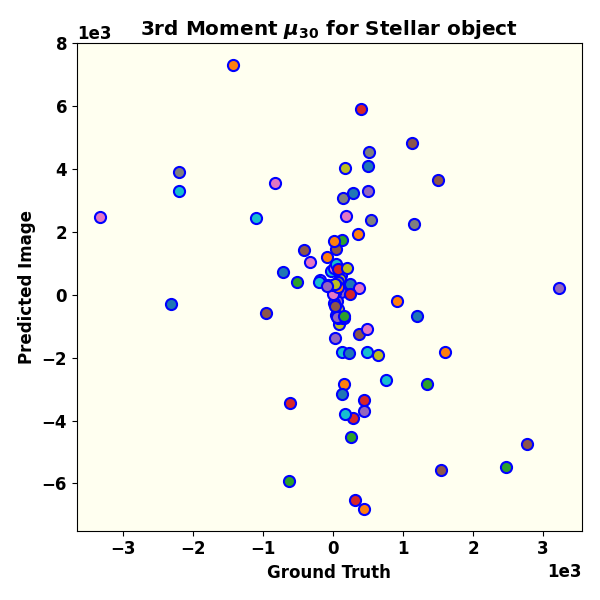
\includegraphics[width=\linewidth]{fig/moments/mom6.png}
		\caption{The 3rd order moment $\mu_{30}$.}
		\label{fig:mom7}
	\end{subfigure}\hfill
	\begin{subfigure}{0.50\linewidth}
		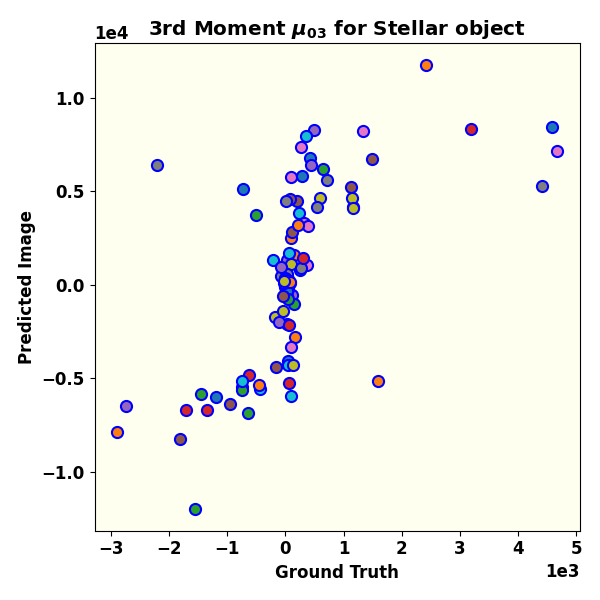
\includegraphics[width=\linewidth]{fig/moments/mom7.png}
		\caption{The 3rd order moment $\mu_{03}$.}
		\label{fig:mom8}
	\end{subfigure}\hfill
	\begin{subfigure}{0.50\linewidth}
		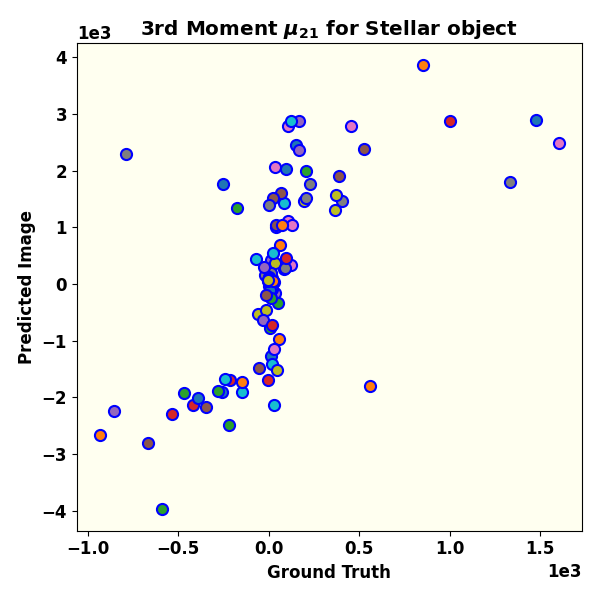
\includegraphics[width=\linewidth]{fig/moments/mom8.png}
		\caption{The 3rd order moment $\mu_{21}$.}
		\label{fig:mom9}
	\end{subfigure}\hfill
	\begin{subfigure}{0.50\linewidth}
		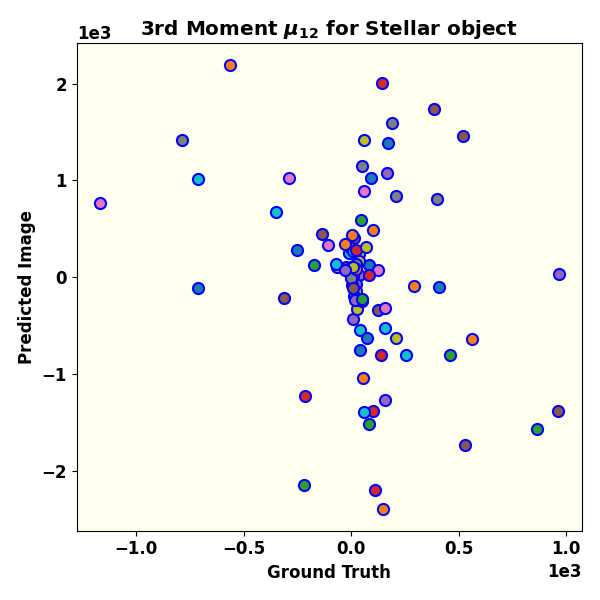
\includegraphics[width=\linewidth]{fig/moments/mom9.png}
		\caption{The 3rd order moment $\mu_{12}$.}
		\label{fig:mom10}
	\end{subfigure}\hfill
	\caption{This set of figures shows all the 3rd-order central moments for ground truth and predicted images generated by trained GAN. It calculates the skewness and evaluates the brightness distribution of images.}
	\label{fig:moments}
\end{figure*}



First, Salt and Pepper noise is introduced at a rate of \(\alpha\) (usually 0.5\%). Then, the images are resized and their mean is subtracted. A two-dimensional Fast Fourier Transform, along with a Fourier shift, is applied, yielding a complex number for each pixel. Since II does not measure phase, the absolute value is calculated (as shown in Fig.~\ref{fig:ft} on both linear and logarithmic scales for visualization). 

Next, sparse sampling is introduced via pixel-wise multiplication between the absolute-valued Fourier-transformed image (Fig.~\ref{fig:ft}) and the sparse sampling map (Fig.~\ref{fig:base}). The result is a map in the Fourier plane featuring several ellipses, which is also referred to as the sparse sampling map (Fig.~\ref{fig:ft_base}). This map represents the sparse sampling for Fig.~\ref{fig:image}, corresponding to the source observed with four telescopes (Fig.~\ref{fig:teles}). 

Finally, the pixels are normalized and converted to 8-bit integers. This image represents the sparsely sampled complex visibility as it can be measured with II. The image shown in Fig.~\ref{fig:ft_base} serves as the input for the GAN, which also requires the corresponding ground truth image. Consequently, the simulated stars are resized using the same algorithm and converted to 8-bit integers to reduce bias. The GAN must have access to the ground truth corresponding to each input image; therefore, the input and ground truth images are merged side-by-side (as shown in Fig.~\ref{fig:GANinput}) and used to train the GAN. This procedure is applied to all simulated stars, with 10\% used as test data, 10\% as validation data, and the remaining 80\% as training data.


\subsection{GAN Architecture}
The GAN used in this work is based on pix2pix, which utilizes a conditional GAN (cGAN) as discussed in the previous section \cite{isola2017image}. This architecture is highly robust and has already been applied to various problems. For instance, the TensorFlow tutorials\footnote{\url{https://www.tensorflow.org/tutorials/generative/pix2pix}} demonstrate its application to a dataset of architectural facades. However, to adapt the pix2pix GAN for the phase retrieval problem, some modifications are necessary. The network is implemented using the TensorFlow library \cite{abadi2016tensorflow}, calculations are performed with scipy \cite{virtanen2020scipy}, and plots are generated with matplotlib \cite{4160265}.

\subsection{Hyperparameter Tuning}
The GAN used in this work depends on several parameters, which are explained briefly below (for a more in-depth discussion, see \cite{murphy2022probabilistic}).

The learning rate of the optimizer determines how much the model updates its parameters with each iteration. A learning rate that is too small may lead to underfitting, while one that is too large can render the model unstable. Therefore, selecting an appropriate learning rate is crucial \cite{murphy2022probabilistic}. Figure~\ref{fig:Plot_learning_rate_loss} illustrates the effect of different learning rates on both the Generator and Discriminator losses. As expected, lower learning rates result in fewer outliers in the loss functions, indicating more stable updates. Although all models eventually stabilize at a similar level, lower learning rates are preferred.

The kernel size refers to the dimensions of the convolutional kernel used in the network, determining how many pixels are combined to produce a new pixel. A larger kernel size can capture features spanning several pixels, but it may also incorporate unrelated features. As shown in Figure~\ref{fig:Plot_kernel_size_loss}, the kernel size does not have a significant impact on the loss functions; however, smaller kernel sizes tend to produce more outliers, suggesting that either the Generator or Discriminator may gain an advantage. Therefore, a kernel size of 5 is preferred.

The amount of noise is controlled by two parameters, \(\alpha\) and \(\beta\), which indicate the percentage of pixels altered to either black or white—hence the term Salt and Pepper noise. Here, \(\alpha\) is applied to the real image, while \(\beta\) is applied to the generated image. Different ratios \(\frac{\alpha}{\beta}\) can lead to varying model performance; however, our results indicate that distinct noise rates do not significantly affect the loss functions. Figure~\ref{fig:Plot_noise_loss} shows the loss functions for smaller images (64 × 64), and due to the negligible impact, this analysis was not repeated for larger images.

The batch size defines the number of images processed simultaneously by the network. Smaller batch sizes have been observed to improve generalization \cite{prince2023understanding}. As illustrated in Figure~\ref{fig:Plot_batchsize_loss}, processing two images at once results in fewer outliers. However, because a larger batch size significantly increases training time, a batch size of 1 is used.

When training GANs, one strategy to potentially boost performance is to give the Discriminator an advantage by increasing its number of training steps before returning to the Generator's training. While this can lower the Discriminator loss—as shown in Figure~\ref{fig:Plot_discrep_loss}—it also increases training time and leads to a slight rise in the Generator loss. Since the generated images do not noticeably improve with additional Discriminator training, both networks are typically trained with the same number of steps.

Finally, the degree of sparse sampling can be varied to provide the model with access to more pixels. Increasing the number of telescopes results in more baselines and, consequently, more available pixels. Figure~\ref{fig:Plot_telescopes_loss} shows the loss functions for different numbers of telescopes. There is a significant disparity in performance, partly because the relationship between telescopes and baselines is not linear. For example, the Fourier plane can be sampled sixfold when using four telescopes compared to using only two. In the case of two telescopes, both the Generator and Discriminator exhibit less smooth training, as indicated by the outliers. Performance improves with three telescopes and becomes very promising with four. Overall, the degree of sparse sampling appears to have the most pronounced effect of all the hyperparameters.
\DIFaddbegin 

\DIFaddend \section{\DIFdelbegin \DIFdel{The }\DIFdelend \DIFaddbegin \DIFadd{Images }\DIFaddend Reconstructed \DIFdelbegin \DIFdel{Image with }\DIFdelend \DIFaddbegin \DIFadd{by the }\DIFaddend GAN}
In this section, we begin by discussing phase retrieval using hyperparameters, as mentioned earlier, followed by an analysis in which multiple sources are trained simultaneously. The best performance for image reconstruction has been observed with a learning rate of \(2 \cdot 10^{-4}\), a kernel size of 5×5, and equal noise percentages applied to both the original and generated images. A batch size of 1 is used, and equal training is provided to both the Discriminator and the Generator.

\subsection{\DIFdelbegin \DIFdel{The }\DIFdelend Predicted Image \DIFdelbegin \DIFdel{with }\DIFdelend \DIFaddbegin \DIFadd{from the }\DIFaddend Trained GAN}
Figure~\ref{fig:GAN} demonstrates the success of the GAN in training a model for Intensity Interferometry (II) to reconstruct images of fast-rotating stars. The GAN was trained on the training datasets for 60,000 steps and subsequently tested on various validation datasets to produce predicted images of a fast-rotating star. In Fig.~\ref{fig:GAN}, four combined images illustrate the GAN's performance in reconstructing the star’s shape, size, and brightness distribution using II.
\begin{itemize}
\item{The left panel shows the signals collected from six baselines, which serve as the input for the Generator during training.}
\item{The first middle panel displays the real image, or ground truth, which the Discriminator uses to distinguish between real images and those generated by the Generator. During training, the GAN aims to replicate these ground truth images.}
\item{The second middle panel presents the reconstructed, or predicted, image produced by the trained GAN, highlighting its success in image reconstruction.}
\item{The right panel shows the difference between the ground truth and the predicted image, with a smaller difference indicating higher precision in image reconstruction.}
\end{itemize}
The predicted images in Fig.~\ref{fig:GAN} yield positive results, accurately conveying visual information about the source's size, shape, and brightness distribution across its surface using only six baselines. However, further improvements can be achieved by increasing the number of telescopes to maximize coverage of the \DIFdelbegin \DIFdel{(u, v) }\DIFdelend \DIFaddbegin \DIFadd{$(u, v)$ }\DIFaddend plane, making the existing and upcoming Cherenkov Telescope Array Observatory (CTAO) an ideal candidate for this approach.
\subsection{Evaluation of GAN using Moments}
The reconstructed images are visually compelling, demonstrating the GAN's effectiveness in using II to reconstruct images. However, visual assessment alone is insufficient; statistical evaluation is necessary to rigorously validate the results. To achieve this, we employ image moments as a statistical method. Image moments capture key properties of the reconstructed objects—such as shape, size, and intensity distribution—by quantifying features like position, orientation, and brightness distribution. By comparing the moments of the GAN-generated images to those of the ground truth, we can objectively assess the consistency and accuracy of the reconstruction. This approach provides a reliable framework for evaluating reconstruction quality, as image moments can reveal subtle differences in geometric and intensity properties that might not be apparent through visual inspection alone.

The raw moment $M_{ij}$ of an image \DIFdelbegin \DIFdel{I(x, y) }\DIFdelend \DIFaddbegin \DIFadd{$I(x, y)$ }\DIFaddend is defined as \citep{hu1962visual}
\begin{equation}
	M_{ij} = \sum_{x} \sum_{y} x^i y^j I(x, y).
	\label{eqn:Mom}
\end{equation}

The zeroth order raw moment, \DIFdelbegin \DIFdel{known as the }\DIFdelend \DIFaddbegin \DIFadd{or }\DIFaddend monopole, represents the total intensity of an image. It is computed by summing all pixel values across the image, yielding an overall intensity measure. In this context, analyzing the monopole provides the total flux of fast-rotating stars. According to eqn.~\ref{eqn:Mom}, the monopole of an image is calculated as:
\begin{equation}
	M_{00} = \sum_{x} \sum_{y} I(x, y).
\end{equation}
Figure~\ref{fig:mom1} displays the monopole values for 50 reconstructed images. The plot reveals a linear relationship between the monopole of the ground truth (real image) on the x-axis and that of the predicted (reconstructed) image on the y-axis, consistent across sources of varying shapes and sizes. This linearity confirms that the predicted images have an overall intensity (flux) that closely matches the ground truth. However, while the monopole effectively represents the total brightness, it does not provide information about the position, shape, size, or detailed brightness distribution of the fast-rotating stars. For these aspects, higher-order moments are necessary.
%%%%%%%%%%%%%%This is original %%%%%%%%%%%%%%%%%%%%%
%To be decided%%%%%%%
The center of mass for the fast-rotating star or any other stellar object is calculated using the centroid (x-centroid and y-centroid). It represents the spatial position of the image and is calculated using first-order raw moment and monopole. The formulation of centroid along the x and y directions is
\begin{equation}
	\begin{aligned}
		&m_x = \frac{\sum_{x} x I(x,y)}{\sum_{x} \sum_{y} I(x, y)} = \frac{M_{10}}{M_{00}} \\
		&m_y = \frac{\sum_{y} y I(x,y)}{\sum_{x} \sum_{y} I(x, y)} = \frac{M_{01}}{M_{00}}
	\end{aligned}  
\end{equation}
Fig.~\ref{fig:mom2} and Fig.~\ref{fig:mom3} show the comparison of the x-centroid and y-centroid for 50 predicted images with respect to ground truths, respectively. The clustering of centroids in a given scale range for all the results explains that the reconstructed image correctly represents the spatial location of the fast-rotating star compared with the ground truth.
%%%%%%%%%%%%%%%%%%%%%%%%%%%%%%%%%%%%%%%%%%

%%%%%%%%%%This portion is generated by ChatGPT%%%%%%%%%%
%%%%To be decided depending on Nitu's reply%%%%

The center of mass of a fast-rotating star, or any stellar object, is determined by its centroid, which provides the x and y coordinates representing the spatial position of the image. This centroid is computed using the first-order raw moments in conjunction with the monopole (the zeroth-order moment). The formulations for the centroid along the x and y directions are given by:
\begin{eqnarray}
&&x_c = \frac{M_{10}}{M_{00}} = \frac{\sum_{x,y} x \cdot I(x,y)}{\sum_{x,y} I(x,y)} \nonumber \\
&&y_c = \frac{M_{01}}{M_{00}} = \frac{\sum_{x,y} y \cdot I(x,y)}{\sum_{x,y} I(x,y)}
\end{eqnarray}
Here, \(I(x,y)\) represents the intensity at pixel \((x,y)\), \(M_{00}\) is the monopole (total intensity), and \(M_{10}\) and \(M_{01}\) are the first-order raw moments along the x and y axes, respectively. This formulation accurately captures the spatial center of mass of the stellar object in the image.

Fig.~\ref{fig:mom2} and Fig.~\ref{fig:mom3} compare the centroids ($x_{c}$, $y_{c}$)of 50 predicted images with their corresponding ground truths, respectively. The clustering of centroids within a specific scale range across all results indicates that the reconstructed images accurately represent the spatial location of the fast-rotating star relative to the ground truth.

%%%%%%%%%%%%%%%%%%%%%%%%%%%%%%%%%%%%%%%%%%%%
Furthermore, these calculated centroids are instrumental in analyzing the shape, size, and brightness distribution of fast-rotating stars using higher-order image moments. To this end, the central moment of an image is calculated according to:
\begin{equation}
	\mu_{pq} = \frac{1}{M_{00}}\sum_{x} \sum_{y} (x - x_c)^p (y - y_c)^q I(x, y).
\end{equation}
The sum of \(p\) and \(q\) defines the order of the central moment. 

Figure~\ref{fig:struc} presents the second-order central moments (\(\mu_{11}, \mu_{20}, \mu_{02}\)), which are used to study the structure of a fast-rotating star along the line of sight (as explained in the upcoming subsection). All three plots demonstrate a linear relationship in the second-order moments, similar to the monopole, thereby confirming the success of applying the GAN to reconstruct images with II.

The brightness distribution is characterized by the skewness of the image, which is quantified by calculating the third-order central moments (\(\mu_{30}, \mu_{03}, \mu_{21}, \mu_{12}\)). Figure~\ref{fig:moments} presents all third-order moments for both the ground truth and the reconstructed image. The skewness along the x and y axes (\(\mu_{30}\) and \(\mu_{03}\)) appears acceptable, as shown in Fig.~\ref{fig:mom7} and Fig.~\ref{fig:mom8}, where a linear relationship exists between the ground truth and predicted images. However, the other higher-order moments (\(\mu_{21}\) and \(\mu_{12}\))—particularly \(\mu_{12}\), as depicted in Fig.~\ref{fig:mom9} and Fig.~\ref{fig:mom10}—do not align as well. This indicates that further improvement is possible and should be investigated.

\subsection{The reconstructed Parameters for object}
The centroids \((x_c, y_c)\) indicate only the center of the fast-rotating star and its spatial location in the image. In contrast, the second-order central moments determine the orientation, semi-major axis, and eccentricity relative to the source's center \citep{teague1980image}. These moment-based parameters fully describe the two-dimensional ellipse that fits the image data.

The orientation of a fast-rotating star along the line of sight is defined in terms of second-order central moments as
\begin{equation}
	\theta = \frac{1}{2}\arctan \big(\frac{2\mu_{11}}{\mu_{20} - \mu_{02}}\big).
	\label{eqn:orn}
\end{equation}
The semi-major and semi-minor axes of the stellar object are computed using the second-order central moments and are denoted as \(a\) and \(b\), respectively.
\begin{equation}
	\begin{aligned}
		&a = 2\sqrt{mp + \delta} \\
		&b = 2\sqrt{mp - \delta}
	\end{aligned}
	\label{eqn:semi}
\end{equation}
where,
\begin{equation}
	mp = \frac{\mu_{20} + \mu_{02}}{2}
	\label{eqn:mp}
\end{equation}
and
\begin{equation}
	\delta = \frac{\sqrt{4\mu_{11}^2 + (\mu_{20} - \mu_{02})^2}}{2}.	
	\label{eqn:delta}
\end{equation}
Using the calculated axis values, the eccentricity of the fast-rotating star is determined as:
\begin{equation}
	e = \sqrt{1 - a/b}.
	\label{eqn:eccen}
\end{equation}
Equations~\ref{eqn:orn}-\ref{eqn:eccen} describe the elliptical nature of the stellar object (in this case, a fast-rotating star) and provide information on its shape and size, depending on the computed values. In contrast, the brightness distribution is characterized by skewness, which is quantified using third and higher-order moments.
\DIFaddbegin 

\DIFaddend \section{Conclusion}
\DIFaddbegin 

\DIFaddend Intensity Interferometry (II) is re-emerging as a promising technique to overcome the challenges \DIFdelbegin \DIFdel{associated with Amplitude Interferometry }\DIFdelend \DIFaddbegin \DIFadd{of very long baseline interferometry }\DIFaddend in the optical wavelength range.  \DIFdelbegin \DIFdel{This resurgence is bolstered by advanced facilities at Imaging Cherenkov Telescope Arrays (ICTAs), which capture high-resolution images using large apertures and sensitive photon detectors capable of resolving signals on the nanosecond timescale \mbox{%DIFAUXCMD
\cite{dravins2013optical}}\hskip0pt%DIFAUXCMD
. The Major Atmospheric Gamma Imaging Cherenkov Telescope (MAGIC), one of the world's leading CTAs, is now being employed for II, observing stellar objects with its 17-meter diameter mirror \mbox{%DIFAUXCMD
\cite{lorenz2004status}}\hskip0pt%DIFAUXCMD
. MAGIC has already demonstrated the potential of II by measuring and comparing the diameters of individual stars \mbox{%DIFAUXCMD
\cite{abe2024performance}}\hskip0pt%DIFAUXCMD
. Other existing arrays, such as the Very Energetic Radiation Imaging Telescope Array System (VERITAS) and the High Energy Stereoscopic System (HESS), are also advancing their II capabilities during periods when gamma-ray observations are not in progress \mbox{%DIFAUXCMD
\cite{kieda2021veritas, zmija2022optical}}\hskip0pt%DIFAUXCMD
. Future observations, enabled by more advanced and sensitive instrumentation as well as the upcoming CTAO, promise to extend the boundaries of optical observations further.
}%DIFDELCMD < 

%DIFDELCMD < %%%
\DIFdelend However, \DIFdelbegin \DIFdel{II faces a significant drawback: it }\DIFdelend \DIFaddbegin \DIFadd{compared to radio-interferometry, optical interferometry faces an important hurdle: photon correlation }\DIFaddend captures only the magnitude of the \DIFdelbegin \DIFdel{signal via photon correlation}\DIFdelend \DIFaddbegin \DIFadd{interferometric signal}\DIFaddend , resulting in a loss of phase information.
\DIFdelbegin \DIFdel{This }\DIFdelend \DIFaddbegin 

\DIFadd{This work addresses the }\DIFaddend challenge of phase retrieval in II \DIFdelbegin \DIFdel{has been effectively addressed through machine learning techniques, particularly with }\DIFdelend \DIFaddbegin \DIFadd{using a machine-learning technique, specifically a }\DIFaddend conditional Generative Adversarial \DIFdelbegin \DIFdel{Networks }\DIFdelend \DIFaddbegin \DIFadd{Network }\DIFaddend (cGAN). Our study demonstrates that applying cGAN to II data successfully recovers the size, shape, and brightness distribution of a fast-rotating star. Evaluations based on image moments—specifically, the monopole, second, and third-order moments—support the effectiveness of cGAN in achieving accurate image reconstruction from a \DIFdelbegin \DIFdel{one-night }\DIFdelend simulation of II \DIFdelbegin \DIFdel{using six baselines.  
A critical }\DIFdelend \DIFaddbegin \DIFadd{from a single site with four telescopes.  
}

\DIFadd{While the results of this study highlight the significant potential of machine learning, and in particular cGAN, for image reconstruction in II, several aspects require further refinement. First, an important }\DIFaddend factor in the reconstruction process is the extent of Fourier plane coverage, which depends on the number of available telescopes and the total observing time. With \DIFdelbegin \DIFdel{a full night of observation using }\DIFdelend \DIFaddbegin \DIFadd{more than }\DIFaddend four telescopes, \DIFdelbegin \DIFdel{the brightness distribution }\DIFdelend \DIFaddbegin \DIFadd{more complicated systems }\DIFaddend could be reconstructed\DIFdelbegin \DIFdel{with even greater precision}\DIFdelend . Future work might explore different observatory layouts to assess their impact on image reconstruction quality\DIFdelbegin \DIFdel{, such as integrating the Southern Cherenkov Telescope Array (CTA) with MAGIC.  }%DIFDELCMD < 

%DIFDELCMD < %%%
\DIFdel{While the results of this study highlight the significant potential of machine learning—particularly cGAN—for image reconstruction in II, several aspects require further refinement. First, }\DIFdelend \DIFaddbegin \DIFadd{.  Second, }\DIFaddend detector efficiencies, which impact the signal-to-noise ratio (SNR) of actual observational data, have not yet been incorporated; addressing these factors will be crucial for more accurate SNR estimation.  \DIFdelbegin \DIFdel{Second}\DIFdelend \DIFaddbegin \DIFadd{Third}\DIFaddend , exploring and comparing alternative methods for image generation could reveal approaches that outperform cGAN in reconstructing stellar images with II. \DIFdelbegin \DIFdel{Third}\DIFdelend \DIFaddbegin \DIFadd{Fourth}\DIFaddend , experimenting with different loss functions could provide additional insights into reconstruction quality. Although further testing is needed to refine the GAN and enhance its robustness and reliability, our findings suggest that machine learning is a promising approach for phase reconstruction in II.


\bibliographystyle{mnras}
\bibliography{refs}

\end{document}
